\documentclass[a4paper, 6pt, landscape]{scrartcl}
\usepackage[german]{babel}
\usepackage[utf8]{inputenc}
\usepackage{multicol}
\usepackage{geometry}
\usepackage{graphicx}
\usepackage{wrapfig}
\usepackage{enumitem}
\usepackage{fancyhdr}
\usepackage{index}
\usepackage{sectsty}
\usepackage{mwe}
\usepackage{comment}
\usepackage{titlesec}
\usepackage[dvipsnames]{xcolor}
\usepackage{amsmath}
\usepackage{amssymb}
\usepackage{listings}
\usepackage{helvet}
\renewcommand{\familydefault}{\sfdefault}
\usepackage{pgfplots}

%Define Math Commands:
\newcommand*{\field}[1]{\mathbb{#1}}%
\newcommand{\Mod}[1]{\ (\mathrm{mod}\ #1)}

%Image Folder:
\graphicspath{{../img/}}

%format
\geometry{top=0.4cm,left=0.5cm,right=0.5cm,bottom=0.4cm}
\setlist{topsep=0pt, leftmargin=5mm, nolistsep}

% Code Snippets

\definecolor{javared}{rgb}{0.6,0,0} % for strings

\lstset{
language=C,
basicstyle=\fontsize{7}{7} \ttfamily,
keywordstyle=\bfseries\color{RoyalBlue},
stringstyle=\color{javared},
commentstyle=\color{MidnightBlue},
morecomment=[s][\color{MidnightBlue}]{/**}{*/},
tabsize=2,
showspaces=false,
showstringspaces=false,
texcl = true,
rulecolor = \color{black},
breaklines = true,
aboveskip = 0em,
belowskip = 0em
}

\usepackage{minted} % for code blocks

\newcommand{\cpp}[1]{\mintinline{cpp}{#1}}
\newcommand{\python}[1]{\mintinline{python}{#1}}
\newcommand{\sh}[1]{\mintinline{sh}{#1}}
\newcommand{\tex}[1]{\mintinline{tex}{#1}}
\newcommand{\sql}[1]{\mintinline{postgres}{#1}}
\newcommand{\txt}[1]{\mintinline{text}{#1}}

\setminted[cpp]{xleftmargin=15pt,mathescape,linenos,obeytabs,breaklines,tabsize=2,escapeinside=||}
\setminted[python]{xleftmargin=15pt,mathescape,linenos,obeytabs,breaklines,tabsize=2,escapeinside=||}
\setminted[sql]{xleftmargin=15pt,mathescape,linenos,obeytabs,breaklines,tabsize=2,escapeinside=||}
\setminted[sh]{xleftmargin=15pt,mathescape,linenos,obeytabs,breaklines,tabsize=2,escapeinside=||}
\setminted[text]{xleftmargin=15pt,mathescape,linenos,obeytabs,breaklines,tabsize=2,escapeinside=||}
\setminted[tex]{xleftmargin=15pt,mathescape,linenos,obeytabs,breaklines,tabsize=2,escapeinside=||}


\newcommand{\TODO}[1]{\noindent {{\color{red}\fbox{\sffamily \bfseries TODO}} \sffamily #1}}
\newcommand{\FIXME}[1]{\noindent {{\color{green}\fbox{\sffamily \bfseries FIXME}} \sffamily #1}}
\newcommand{\CHECK}[1]{\noindent {{\color{orange}\fbox{\sffamily \bfseries CHECK}} \sffamily #1}}
\newcommand{\CONSIDER}[1]{\noindent {{\color{blue}\fbox{\sffamily \bfseries CONSIDER}} \sffamily #1}}



% Define Section Format
\titleformat{name=\section}[block]
{\sffamily\normalsize}
{}
{0pt}
{\colorsection}
\titlespacing*{\section}{0pt}{0pt}{0pt}

\newcommand{\colorsection}[1]{%
\colorbox{MidnightBlue!40}{\parbox{0.98\linewidth}{\color{black}\thesection\ #1}}}


% Define Subsection Format
\titleformat{name=\subsection}[block]
{\sffamily\small}
{}
{0pt}
{\colorsubsection}
\titlespacing*{\subsection}{0pt}{0pt}{0pt}

\newcommand{\colorsubsection}[1]{%
\colorbox{YellowGreen!50}{\parbox{0.98\linewidth}{\color{black}\thesubsection\ #1}}}

% Define SubSubsection Format
\titleformat{name=\subsubsection}[block]
{\sffamily\small}
{}
{0pt}
{\colorsubsubsection}
\titlespacing*{\subsubsection}{0pt}{0pt}{0pt}

\newcommand{\colorsubsubsection}[1]{%
\colorbox{Goldenrod!50}{\parbox{0.98\linewidth}{\color{black}\thesubsubsection\ #1}}}

% -----------------------------------------------------------------------
\begin{document}
    %	\pagecolor{p}
    %	\color{t}
    \setlength{\columnseprule}{0.4pt}
    %\footnotesize
    \begin{multicols*}{3}
        \tableofcontents
        %! Author = Philipp Emmenegger
%! Date = 30/06/2021
\subsection*{Abkürzungen}
\begin{itemize}
    \item \textbf{ADAM} Adaptive Moment Estimation
    \item \textbf{ANN} Artificial Neural Network
    \item \textbf{KNN} K Nearest Neighbour
    \item \textbf{MSE} Mean Squared Error
    \item \textbf{MLE} Maximum Likelihood Estimation
    \item \textbf{NLP} Natural Language Processing
    \item \textbf{OLS} Ordinary Least Squares
    \item \textbf{PMF} Probability Mass Function (Wahrscheinlichkeitsfunktion)
    \item \textbf{ROC} Receiver Operating Characteristics
    \item \textbf{SGD} Stochastic Gradient Descent 
    \item \textbf{WCSS} within-cluster sum-of-squares
\end{itemize}

\section{Introduction}
\textbf{Artificial Intelligence}
\begin{itemize}
    \item broad concept
    \item different interpretations
    \item we do not have a definition of inteligence
\end{itemize}
\textbf{Statistical machine learning}
\begin{itemize}
    \item Algorithms and applications where computer learn from data
\end{itemize}
\textbf{AGI}
\begin{itemize}
    \item Artificial General Intelligence
    \item Hypothetical computer program that can perform intellectual tasks as well as, or better than a human.
\end{itemize}
\textbf{Turing Test}
\begin{itemize}
    \item Also called imitation game
    \item Tests of a machine's ability to exhibit intelligent behaviour equivalent to, or indistinguishable from that of a human
    \item Has some philosophical problems (Complex problems, humans cant solve / AI must learn to lie)
\end{itemize}
\textbf{Examples of application (today):}
\begin{itemize}
    \item Personalization of news feeds
    \item Product searching and recommendation s on eCommerce platforms
    \item Voice-to-text
    \item Predictive maintenance
\end{itemize}
\subsection{Tasks and Algorithms of Machine Learning}
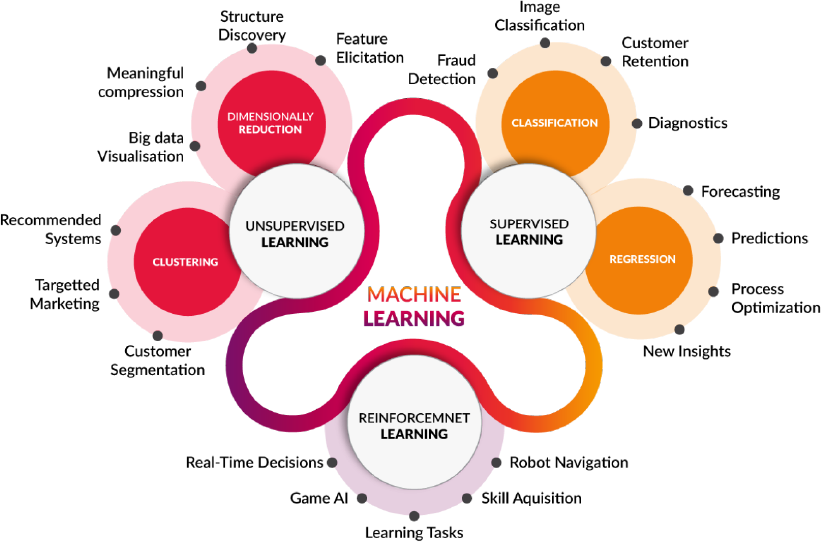
\includegraphics[width=\linewidth]{./img/machine_learning_sections.png}

\subsection{Natural Language Processing (NLP)}
\begin{itemize}
    \item Automated processing of human language (written \& spoken)
    \item Aims to understand and generate human (natural) language
    \item Understanding spoken text is still difficult
    \item Understanding written text became BIG business (search-engines)
    \item Generating human-like conversations is still very hard
\end{itemize}

\subsection{Dialogflow}
\textbf{Intents}
\begin{itemize}
    \item Recognizes the need of a user
    \item Require training to match to user inputs
    \item Follow up Intents (on Success)
    \item Fallback Intents (on Failure)
\end{itemize}
\textbf{Intent Matching (Recognize what your user want)}
\begin{itemize}
    \item For each intent, we provide examples for the various ways the user might communicate it
    \item Dialogflow uses this information to train a machine-learning model to understand not just the examples we've entered, but numerous other phrases that mean the same thing
\end{itemize}
\textbf{Entities/ Entity-Extraction}
\begin{itemize}
    \item Extract information from user inputs
    \item Help to identifiy required intent
    \item System Entities: (Date and time / Numbers / Amounts / Units / etc.)
    \item Developer Entities: defined by list of words (@pizza-type / @drink / etc.)
    \item User Entities: transient, temporary Information based on Conversation
\end{itemize}
\textbf{Dialog}
\begin{itemize}
    \item Linear: Gather a list of information
    \item Non Linear: Using Contexts
\end{itemize}
\textbf{Agents}
\begin{itemize}
    \item handles concurrent conversations with your end-users. It is a natural language understanding module that understands the nuances of human language. 
    \item is similar to a human call center agent
    \item top-level container for settings and data (intents, entities, knowledge, fullfillment..)
\end{itemize}
\textbf{Context}
\begin{itemize}
    \item Each Intent can have Input \& Output Context
    \item Intents are active based on active Context
    \item Expire automatically
\end{itemize}
\textbf{Fulfillment}
\begin{itemize}
    \item Action triggered on fullfilled Intents
    \item e.g. Webhook
\end{itemize}

\subsection{7 Steps of ML}
\begin{enumerate}
    \item Gathering data
    \item Preparing that data
    \item Choosing a model
    \item Training
    \item Evaluation
    \item Hyperparameter tuning
    \item Prediction
\end{enumerate}

\subsection{Algorithms}
\begin{itemize}
    \item \textit{Gradient Descent Algorithm}: linear regression, logistic regression, neural networks
    \item \textit{Distance-based Algorithm}: KNN, k-means
\end{itemize}
        \section{Natural Language Processing (NLP)}
\subsection{The 4 Key-Ingredients of Machine Learning}
\textbf{1. Data (Input)}
\begin{itemize}
    \item Dataset (Input-Vektor), bestehend aus Features ($X$) und Labels ($Y$).
    \item Pre-Processing Pipe-Line including cleansing, feature-engineering, data augmentation etc.
    \begin{itemize}
        \item \textbf{cleansing}: identifying and correcting errors in the dataset. z.B. Rechtschreibefehler in Text erkennen und korrigieren (mögliches korrektes Wort vorschlagen)
        \item \textbf{feature-engineering}: the process of using domain knowledge to extract features (characteristics, properties, attributes) from raw data. Nicht nur Rohdaten, sondern auch noch Features extrahieren (nicht nur Katze vorschlagen, sondern auch Verbindung von Katze zu Säugetier herstellen). Damit ML Modell mit Features weiterarbeiten kann (z.B. Wörter in One-Hot-Rep. darstellen)
        \item \textbf{Data-Augumentation}: Man hat gewisse Daten (z.B. Sammlung von Katzenfotos), damit man gut Machine-learning machen kann benötigt man viele Daten $\rightarrow$ vorhandene Bilder manipulieren (schwarz/weiss, spiegeln, etc.) um aus einem Bild möglichst viele andere zu erstellen damit man mehr Inputs hat
    \end{itemize}
\end{itemize}
\textbf{2. Cost-Function (Loss)}
\begin{itemize}
    \item Formal mathematical expression for good / bad
    \item Commonly Mean Squared Error (MSE)
    \item \textit{Beispiel}: 2 Fotos vorhanden (Katzen und Hunde) $\rightarrow$ wenn Katze als Hund erkannt wird, ist das sehr schlecht und muss dem Computer mitgeteilt werden (Mathematische Funktion wie gut oder schlecht Ergebnis war)
    \item auch Fehler oder Residual genannt (Differenz zwischen Vorhersage $\hat{y}$ und Wirklichkeit $y$ )
\end{itemize}
\textbf{3. Model}
\begin{itemize}
    \item From linear model: $\hat{y_i} = ax_i + b$
    \item To complicated million parameter neural networks
    \item Different tasks require different models (regression / decision tree)
    \item Aus einem Input wird (über eine mathematische Funktion) ein Output generiert
\end{itemize}
\textbf{4. Optimization Procedure (Optimizer)}
\begin{itemize}
    \item Algorithm that changes the parameters of the model that the cost-function is minimized.
    \item E.g. \textit{Stochastic Gradient Descent (SGD), ADAM, RMSProp...}
    \item Model Trainieren mit verschiedenen Parametern, etc.
\end{itemize}

\subsection{More ingredients}
For successful ML, there are many more ingredients:\\ 
\textbf{5. Performance optimization}
\begin{itemize}
    \item Building of efficient pipe-lines
    \item Folowing tool specific recommendations
\end{itemize}
\textbf{6. Visualization and evaluation of the learning Process}
\begin{itemize}
    \item Learning curves
    \item Performance measures
    \item Tensorboard
\end{itemize}
\textbf{7. Cross-Validation \& Regularization}
\begin{itemize}
    \item Train models that generalize well to unseen data
    \item Estimate the generalization error
\end{itemize}

\subsection{Representation of Words}
Vectors can be used to represent words based on their meaning.
\subsubsection{One-hot representation/ One-hot Encoding}
\begin{itemize}
    \item Vector with a single 1-Value
    \item All other Values are set to 0
    \item Skalarprodukt von Vektoren ergibt IMMER 0
    \item Count the Number of different Words, Define one unique vector per word:
\end{itemize}
\textit{Dini Mom isch fett.}\\
Dini: $\begin{bmatrix} \textcolor{red}{1}\\ 0\\ 0\\ 0\\ 0\end{bmatrix}$
Mom: $\begin{bmatrix} 0\\ \textcolor{red}{1}\\ 0\\ 0\\ 0\end{bmatrix}$
isch: $\begin{bmatrix} 0\\ 0\\ \textcolor{red}{1}\\ 0\\ 0\end{bmatrix}$
fett: $\begin{bmatrix} 0\\ 0\\ 0\\ \textcolor{red}{1}\\ 0\end{bmatrix}$
'.': $\begin{bmatrix} 0\\ 0\\ 0\\ 0\\ \textcolor{red}{1}\end{bmatrix}$\\ 
\textbf{Disadvantages:}
\begin{itemize}
    \item Very high dimensional vector space (1 Dimension / unique Word)
    \item Sparse Representation: Eech vector has a single 1 and $N$ Zeroes. (Memory Inefficient)
    \item No Generalization: All words are unrelated to each other.
    \item Does not capture any aspect of the meaning of a word
\end{itemize}

\subsubsection{Indexing}
Make a list of words (optionally alphabetically). Use the index to represent each word.\\ 
\textbf{Example:}\\
\textit{Dini Mom isch fett.}\\ 
Dini: $0$, Mom: $1$, isch: $2$, fett: $3$, '.': $4$
\begin{itemize}
    \item Dense Equivalent of one-hot encoding
    \item Indexes are not more useful that one-hot vectors
    \item Often used as preprocessing step
    \item Indices / One-Hot Vectors are fed into a network which learns more useful representations
\end{itemize}

\subsubsection{Distributed Representation}
\begin{itemize}
    \item Words that occur in similar contexts (neighboring words) tend to have similar meanings
    \item Similar words share similar representations
    \item Distributed representations can be learned
\end{itemize}
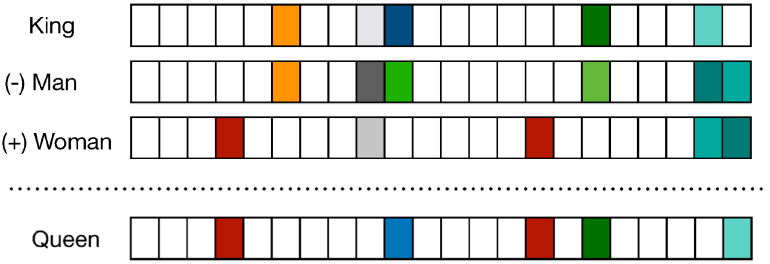
\includegraphics[width=.8\linewidth]{./img/distributed_representation.png}\\
\textbf{Words to Vectors:}
\begin{itemize}
    \item Mathematical function maps word to high dimensional Vector
    \item In neural networks, this function is implemented in the Embedding Layer
\end{itemize}
\textbf{Advantage of Vectors}
\begin{itemize}
    \item Good embedding maps simiar/related words to similar regions of the vector space
    \item Dot-Product (Skalarprodukt) is a measure of similarity
    \item Possible to add/subtract vectors
\end{itemize}
\textbf{Calculate Similarities between words}
Dot-Product (Skalarprodukt) of 2 Vectors:
\begin{itemize}
    \item maximal when parallel (0\textdegree) (1 with norm (length) 1)
    \item zero when orthogonal/ senkrecht (90\textdegree)
    \item minimal (negative) when opposite directions (180\textdegree) (-1 with norm (length) 1)
\end{itemize}
\textbf{Why make it sense to normalize the vector representations \TODO{allenfalls normalisieren erklären}}
\begin{itemize}
    \item Skalarprodukt wird auf 1 "Normalisiert" $\rightarrow$ somit muss Skalarprodukt in Formel nicht mehr ausgerechnet werden
    \item damit norm-Vektor nicht immer neu ausgerechnet werden muss, sondern nur noch verwendet werden kann
\end{itemize}
\textbf{Cosine Distance}
\begin{itemize}
    \item Way to calculate how similar two words (vectors) are
\end{itemize}
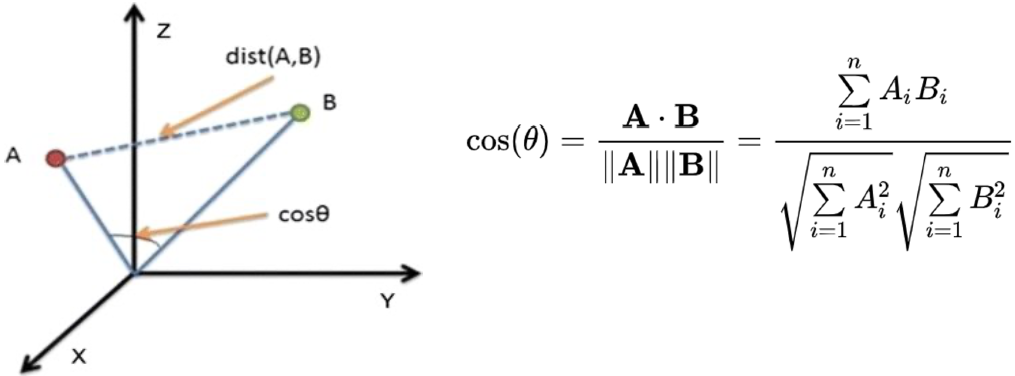
\includegraphics[width=\linewidth]{./img/cosine_distance.png}

\subsubsection{Cosine-Distance vs. Cosine-Similarity}
\begin{itemize}
    \item cosine similarity is a similarity metric between vectors
    \item Je grösser die Cosine-Distanz wird, desto kleiner wird auch die Cosine-Similarity
    \item Je kleiner die Cosine-Distanz wird, desto höher wird auch die Cosine-Similarity
    \item Je kleiner $cos(\theta)$, desto höher die Similarity \& desto kleiner  die Distance
    \begin{itemize}
        \item \textit{Cosine similarity range}: $-1$ meaning exactly opposite, 1 meaning exactly the same, 0 indicating orthogonality (senkrecht)
    \end{itemize} 
    \item if 2 vectors are perfectly the same then similarity is 1 (angle=0) and thus, distance is 0 (1-1=0)
    \item \textbf{Cosine-Similarity}: $cos(\theta) = \frac{a * b}{|a|*|b|} \rightarrow$ Winkel zwischen $P_1$ \& $P_2$
    \item \textbf{Cosine-Distance}: $1 - CosineSimilarity$
\end{itemize}
        \section{Probability}
\subsection{Random Variables}
\begin{itemize}
    \item Values depend on outcomes of a random phenomenon
    \item Random variable $X$ is a variable that takes a numerical value $x$, which depends on a random experiment
    \item \textbf{Discrete:} $X$ takes any of a finite set of values ${1.5, 2.123, 6.2, 10}$
    \item \textbf{Continous:} $X$ takes any alue of an uncountable range e.g. real numbers from an interval
\end{itemize}
\textbf{Best we can know}
\begin{itemize}
    \item All possible values
    \item Probability of each value
\end{itemize}
E.g. The discrete random variable $X$ is the number observed when rolling a fair dice.\\ 
$Pr(X=x)$ / $P(x)$: $1/6$ for each possible value (the probability that the random variable X takes the value x)

\subsubsection{Two random variables}
\textbf{Joint Probability}
\begin{itemize}
    \item Joint Properties of two random variables
    \item Defined by the Joint Probability Mass Function
\end{itemize}
E.g. Dice1 = 5 AND Dice2 = 4\\
$P_{XY}(5,4) = 1/36$\\ 
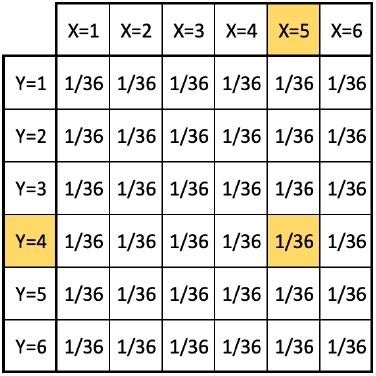
\includegraphics[width=0.5\linewidth]{./img/joint_probability.png} \\
\textbf{Correlated random Variables}
\begin{itemize}
    \item There are events that are not independant
    \item Such random variables are correlated
    \item $X$: observe clouds (0=no, 1=small, 2=big)
    \item $Y$: observe rain (0=no, 1=light, 2=moderate, 3=heavy)
\end{itemize}

\subsubsection{Join Probability/ Independant random Variables}
\begin{itemize}
    \item Joint Probability is the product of the individual probabilities
\end{itemize}
$P(X,Y) = P(X) \cdot P(Y)$ (only if independant)\\ 
$P(X,Y,Z) = P(X) \cdot P(Y) \cdot P(Z)$ (only if independant)

\subsubsection{Conditional Probability}
\begin{itemize}
    \item One variable is no longer random
    \item X is observed, its value is fixed
    \item Calculate the probabilities of Y given X: $P(Y | X)$
\end{itemize}
$P(X, Y) = P(X | Y) \cdot P(Y)$\\ 
$P(X, Y) = P(Y | X) \cdot P(X)$\\
$P(Y | X) = \frac{P(X,Y)}{P(X)}$

\subsubsection{Marginal Probability}
\begin{itemize}
    \item What is the general approach to recover the PMF Pr(X=x) of one random variable, given the joint probability Pr(X,Y) ?
    \item Man kann immer die Summen bilden (siehe Beispiel anhand Tabelle)
    \begin{itemize}
        \item $P(X=1) = Y(1) + Y(2) + Y(3) + Y(4) + Y(5) + Y(6) = 6/36 = 1/6$
    \end{itemize}
    \item Marginal Distribution = Summe einer Dimension (X oder Y)
\end{itemize}

\subsubsection{Bayes Rule}
$P(X|Y) \cdot P(Y) = P(Y|X) \cdot P(X)$\\ 
Therefore:\\
$P(Y|X) = \frac{P(X|Y) \cdot P(Y)}{P(X)}$

\subsubsection{Probability Mass Function (PMF)}
\begin{minipage}{0.6 \linewidth}
The PMF of a discrete random variable is a function $f(x)$ that provides the probability for each value $x$ of a discrete random variable $X$.\\
A PMF specifies a (discrete) \textbf{Probability Distribution} (de: Wahrscheinlichkeitsverteilung). (but often the two terms are used as synonyms.)\\
\textbf{Aus Übung:} density = dursch. hits / nr of samples. Für Warscheinlichkeit Fläche unter der Kurve ausrechnen. Also z.b. Interval [-4,-1] und Density 0.1 = 0.1*3=30\%
\end{minipage}
\begin{minipage}{0.4 \linewidth}
\centering
Graph of a PMF (dice) $f(x)$:\\
\begin{tikzpicture}
    \begin{axis}[
    width=\textwidth,
    height=3cm,
    xmin = 0, xmax = 6,
    ymin = 0, ymax = 1,
    ytick={1/6,1},
    yticklabels={$\frac{1}{6}$,1},
    xtick={1,2,3,4,5,6},
    axis y line=left,
    axis x line=bottom,
    xlabel=$x$, ylabel=$f(x)$, 
    ]
        \addplot[black, only marks] coordinates {
          (1, 1/6)
          (2, 1/6)
          (3, 1/6)
          (4, 1/6)
          (5, 1/6)
          (6, 1/6)
        };
    \end{axis}
\end{tikzpicture}
\end{minipage}
        \section{Data Visualization}
\begin{itemize}
    \item See trends, clusters and patterns in data
    \item Difficult to see in raw data
    \item Detect outliers and unusual groups
    \item Validate Hypothesis/Conjecture/Theory
\end{itemize}
\textbf{Important in a Plot:}
\begin{itemize}
    \item X-Axis / Y-Axis
    \item Title
    \item Scale
    \item Dimensionality of the data 2D / 3D
\end{itemize}
%\textbf{Plot types:}
%\begin{itemize}
%    \item \textit{Line}: trends, movement over time
%    \item \textit{Bar}: categorical data where binning/counting is done
%    \item \textit{Histogram (Häufigkeitsverteilung)}: represents the empirical distribution. number of observations vs bins (range of values)
%    \item \textit{Box \& Violin}: Descriptive Statistics (empirische Daten/Sammlung von Daten durch Tabellen, Kennzahlen und Grafiken übersichtlich darzustellen)
%    \item \textit{Scatter (Punktewolke)}: relationship between two continuous variables. color to encode a third variable
%\end{itemize}

\subsection{Descriptive statistics (Mittelwerte für Boxplots, etc.)}
\textbf{Mean (Normalfall)}
\begin{itemize}
    \item ''normaler'' Durchschnitt
    \item ist stark von Abreissern abhängig resp. Ausreisser verändern Auswertung sehr stark
\end{itemize}
\textbf{Median}
\begin{itemize}
    \item Der Wert, der genau in der Mitte einer Datenverteilung liegt (Bei 10 Punkten ist 5. Punkt der Median)
    \item ist nicht gross abhängig von Ausreissern und kann somit ein genaueres/ repräsentativeres Ergebnis darstellen
    \item wenn Daten Tendenz in eine Richtung haben (damit Ergebnis Aussagekräftig bleibt)
\end{itemize}
\textbf{Percentile}
\begin{itemize}
    \item wird verwendet, wenn andere Werte als die zentralen Werte der Daten gefunden werden müssen \item Während bei der Verwendung des Medians die Daten in zwei gleiche Hälften geteilt werden und der mittlere Wert berechnet wird, bietet die Perzentilmethode die Flexibilität, jeden beliebigen Wert zu berechnen, wenn die Daten zwischen 1 und 100 geteilt werden. 
\end{itemize}
\textbf{Häufig genutzte Percentile}
\begin{itemize}
    \item 50\%-Percentile = Median
    \item 25\%-Percentile = 1. Quantil
    \item 75\%-Percentile = 3. Quantil
\end{itemize}

\subsection{Data Analysis Libraries}
\subsubsection{NumPy}
\begin{itemize}
    \item Package for scientific computing in Python
    \item Multidimensional array object
    \item Routines for fast array operations (sorting, selecting, FFT, linalg, etc)
\end{itemize}

\subsubsection{pandas}
\begin{itemize}
    \item Built on top of NumPy
    \item Routines for accessing tabular data from files (.csv, xls, etc.)
    \item Supports 2-dimensional data (dataframe and series)
    \item Dataframes are something like database tables
\end{itemize}

\subsubsection{MatPlotLib}
\begin{itemize}
    \item Library for visualizing data
    \item Bargraphs, Histograms, Piecharts, Scatter plots, lines, boxplots, heatmaps, etc.
\end{itemize}

\subsubsection{Seaborn}
\begin{itemize}
    \item Extension of MatPlotLib, NumPy and pandas
    \item More user friendly
    \item Plots are aesthetically better
\end{itemize}

\subsubsection{Chart types}
\textbf{Line Plots}
\begin{itemize}
    \item \textit{Bivariate, Continous}
    \item Recognizes trend (pattern of change)
    \item general movement over time of a statistically detectable change
\end{itemize}
\textbf{Bar Chart}
\begin{itemize}
    \item Used for \textit{categorical data}
    \item Counting based on each category (e.g. Apps in AppStore, PlayStore, Windows Store, etc.)
\end{itemize}
\textbf{Histogram (Häufigkeitsverteilung)}
\begin{itemize}
    \item Represents the \textit{empirical distribution} of a variable
    \item Automatically creates bins (interval) along the range of values
    \item Shows vertical bars to indicate the number of observations / bin
\end{itemize}
\textbf{Descriptive Statistics: Box Plots and Violin Plots}\\
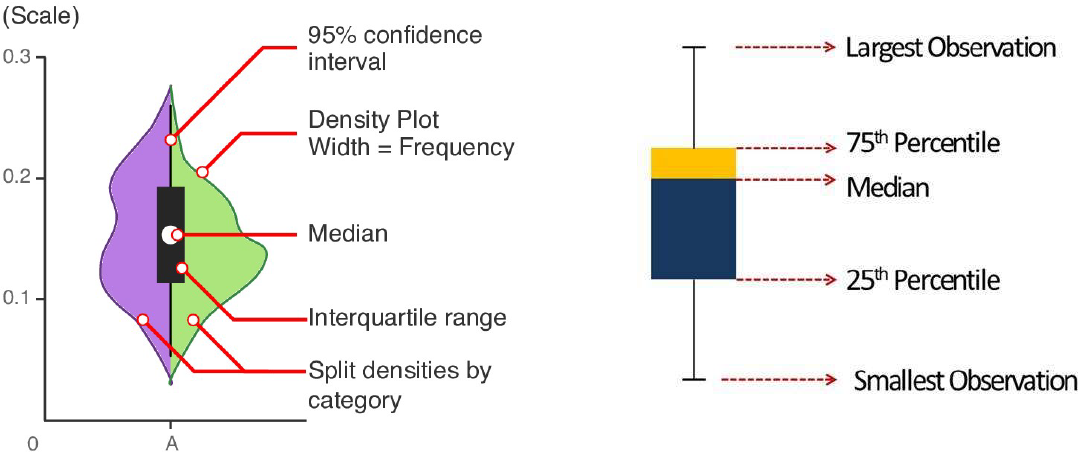
\includegraphics[width=\linewidth]{./img/descriptive_statistics.png}
\textbf{Scatter Plot}
\begin{itemize}
    \item Relationship between two \textit{continous} variables
    \item Helps to get an idea of the degree of correlation between variables
\end{itemize}
        \section{Regression}
\subsection{What is a model?}
In ML, we use the term \textbf{model} for any mathematical function that explains the data:\\ 
$y_i \approx f(x_i) \qquad y_i = f(x_i) + \epsilon_i \qquad \hat{y_i}=a*x_i+b$\\ 
where $\epsilon_i$ is unexplained noise. It is often assumed that $\epsilon_i$ follows a normal distribution.\\ 
Instead of approximating $y_i$, we calculate an \textbf{estimate} $\hat{y_i}$ (y hat) of the usually unknown $y_i$: \\
$\hat{y}_i = f(x)$

\subsubsection{Linear Regression}
\label{sec:lin_reg}
\begin{itemize}
    \item Only consideres a linear relationship between input and output
     \begin{itemize}
         \item z.B. erwachsene Menschen sind grösser als Kinder
     \end{itemize}
     \item Mit Linear Regression können zusammenhänge zwischen 2 und mehr Variablen herausgefunden werden
     \begin{itemize}
         \item z.B. gibt es einen Zusammenhang zwischen Rauch und Lungenkrebs
     \end{itemize}
    \item In the simplest case, $x$ and $y$ are scalars and the linear model therefore has only two free parameters
    \item The goal is to identify $a$ (slope) and $b$ (intercept) for which the linear model best explains the data
    \item $a$ an $b$ are parameters (weights) of the model and can be trained
\end{itemize}
\begin{center}
    $\hat{y}_i = ax_i + b$
\end{center}

\subsubsection{Polynomiale Regression}
%\textbf{HINT:} kubisch $\rightarrow$ 3. Ordnung $\rightarrow$ 4 freie (trainierbare) Parameter ($w$) $\rightarrow$ z.B. $\hat{y} = w1*x^1 + w2*x^2 + w3*x^3 + w0$ (letzter Parameter ist von $x^0$)
%Modell als Gleichung: $\hat{y}_i = \omega_3 \cdot x_i^3 + \omega_2 \cdot x_i^2 + \omega_1 \cdot x_i + \omega_0$

%MSE als math. Gleichung: (siehe auch unten)
%\begin{center}
%    $E = \frac{1}{2N} * \large\displaystyle\sum_{i = 1}^{N}(y_i - (\omega_3 \cdot x_i^3 + \omega_2 \cdot x_i^2 + \omega_1 \cdot x_i + \omega_0))^2$
%\end{center}

\textbf{kubisch}: $\hat{y} = \omega_1*x^1 + \omega_2*x^2 + \omega_3*x^3 + \omega_0 \rightarrow$ 4 (freie trainierbare) Parameter (letzter Parameter ist von $x^0$\\
\textbf{quadratic}: $\hat{y}_i = \omega_2 \cdot x_i^2 + \omega_1 \cdot x_i + \omega_0 \rightarrow$ 3 Parameter\\
\textbf{linear}: $\hat{y}_i = \omega_1 \cdot x_i + \omega_0 \rightarrow$ 2 Parameter\\

\subsubsection{Mean Squared Error (MSE), Residual}
\begin{itemize}
    \item Loss we want to minimize
    \item Usually divided by 2
    \item The difference $e_i$ (Abweichung), is called \textbf{residual}
    \begin{itemize}
        \item The difference between an observed value of the actual value and the value of the predicted value from the regression line
    \end{itemize}
    \item Where $e_i$ is ''unexplained noise''. It is often assumed that $e_i$ follows a normal distribution
\end{itemize}
\begin{center}
    $\hat{y}_i = ax_i + b$\\ 
    $e_i = y_i - \hat{y}_i$ \\ 
    
    $E = \frac{1}{2N} * \displaystyle\sum_{i = 1}^{N} {e_i}^2$\\
    $E = \frac{1}{2N} * \large\displaystyle\sum_{i = 1}^{N}(y_i - \hat{y}_i)^2$
\end{center}

\textbf{Question:} \textit{The MSE is a scalar value calculated using the formula above. If you had to implement a function \python{calc_mse()}, what would be the input parameters of that function?}\\
$E = f(X, Y, a, b)$ ($X$\&$Y$ = Vectors, $a$\&$b$ = Parameters)

\subsubsection{Correlation and Causality}
\begin{itemize}
    \item Correlation is not causality
    \item Correlation refers to the degree to which a pair of variables are linearly related
    \item Linear regression is a tool to detect correlations between two or more variables
    \item Correlation can be quantified using the Pearson correlation coefficient
\end{itemize}


\subsection{The FIT method in scikit-learn LinearRegression class}
The \python{.fit(X, y[, sample_weight])} Method in Scikit-Learn does the training which includes regresion

\begin{minted}{python}
X = np.array([[1, 1], [1, 2], [2, 2], [2, 3]])
y = np.dot(X, np.array([1, 2])) + 3 # y = 1 * x_0 + 2 * x_1 + 3
reg = LinearRegression().fit(X, y)
reg.score(X, y) #> 1.0
reg.coef_ #> array([1., 2.])
reg.intercept_ #> 3.0...
reg.predict(np.array([[3, 5]])) #> array([16.])
\end{minted}

\subsection{Uniform Distribution, Normal Distribution}
\begin{itemize}
    \item Uniform Distribution: horizontale 
    \item Normal Distribution: Glockenkurve
\end{itemize}

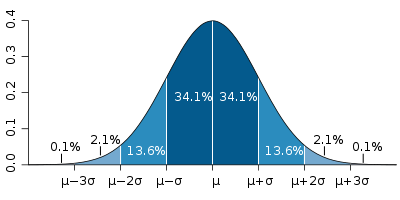
\includegraphics[width=0.8\linewidth]{./img/normal_distribution.png}

\begin{itemize}
    \item 68,27\% aller Werte im Intervall von einer Standardabweichung,
    \item 95,45\% aller Werte im Intervall von zwei Standardabweichungen
    \item 99,73\% aller Werte im Intervall von drei Standardabweichungen
\end{itemize}

\subsection{Seaborns jointplot}

\begin{minipage}{0.5\linewidth}
Der Jointplot ist eine verbindung von zwei Variablen mit bivariaten und univariaten Graphen. Es zeigt die (empirischen) Randverteilungen als Histogramme. Das Ergebnis ist ideal: die Daten (x-Werte) sind gleichmäßig über den gesamten Bereich verteilt (Gleichverteilung in -50/+50), während die Residuen bei 0 zentriert sind (Standardnormalverteilung).
\begin{minted}{python}
    penguins = sns.load_dataset("penguins")
    sns.jointplot(data=penguins, x="bill_length_mm", y="bill_depth_mm")
\end{minted}
\end{minipage}
\begin{minipage}{0.5\linewidth}
    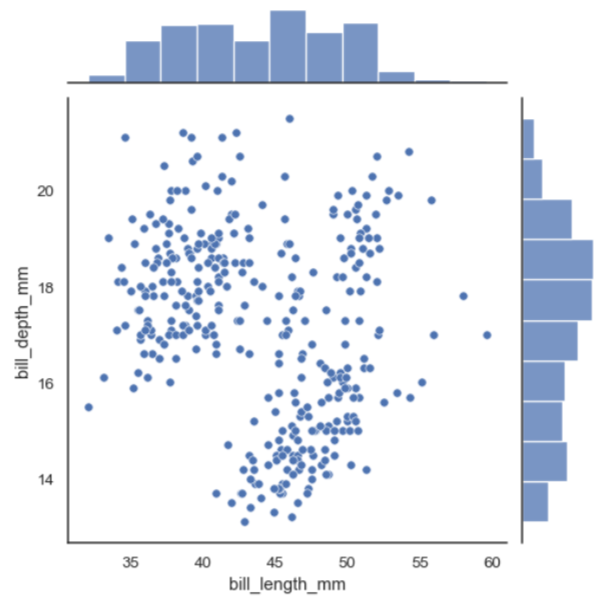
\includegraphics[width=\linewidth]{./img/sns_jointplot.png}
\end{minipage}


\subsection{Pearson Correlation Coefficient}
refers to the degree to which a pair of variables are linearly related. $0\rightarrow$ Kein Zusammenhang / $>0\rightarrow$ positiver Zusammenhang / $<0\rightarrow$ negativer (gegenläufiger) Zusammenhang.\\
\textbf{Achtung}: Beinhaltet keine Aussage über die Kausalität!  

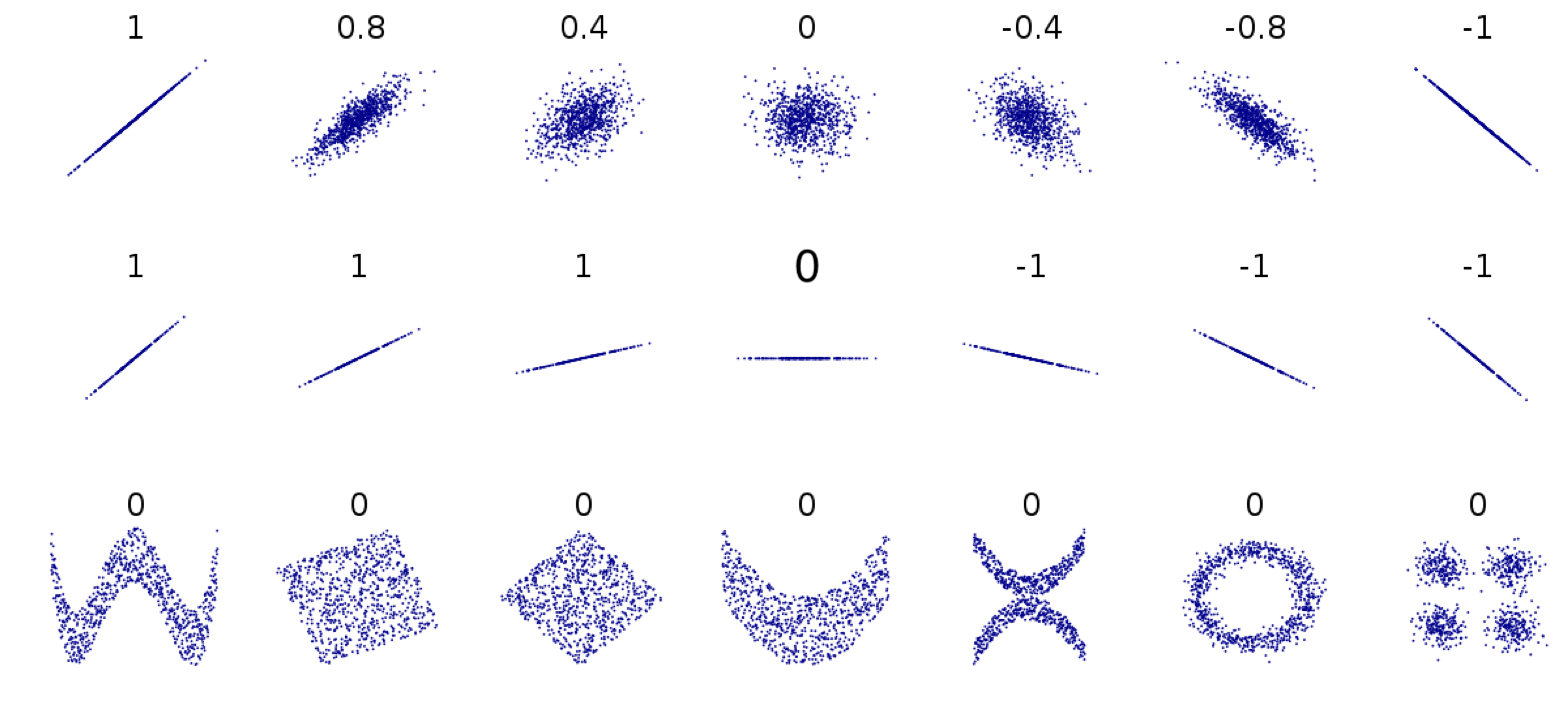
\includegraphics[width=\linewidth]{./img/pearson_correlation_coefficient.png}
        \section{Optimization (Stoachistic Gradient Descent)}
\begin{itemize}
    \item Training or learning in AI often suggests an algorithm performing some sort of optimization
    \item It is the problem of finding a set of inputs to an objective function that results in a maximum or minimum function evaluation
    \item In our examples the \textbf{goal is to minimize the loss function}
\end{itemize}

\subsection{Error-landscape and Parameter-Space}
\textbf{Parameter-Space}: Alle möglichen Kombinationen von Parametern (Gewichte) die möglich sind (AxB)
\textbf{Error-Landscape}: Der Error (Loss), der im Parameter-Space (Error pro einzelne Kombination) entsteht ergibt eine Error-Landscape (E=AxB)

\subsection{Gradient Descent}
Gradient Descent ist ein fundamentaler Optimizer-Algorithmus: Der \textbf{Gradient} (=Steigung/Slope/Gewicht) wird so optimiert, das er in der "tiefsten Punkt" (Descent=Absenkung,Verminderung) in der Error Landscape landet.
\begin{itemize}
    \item Iterative Method to find the optimal values for its parameters
    \item Each iteration, the model parameters are updated such as that the Loss (MSE) is reduced
    \item versucht Optimum herauszuholen (Loss Function (MSE) möglichst klein machen)
    \item führt nur wenige Berechnungen weit entfernt vom Optimum durch und erhöht die Anzahl der Berechnungen ($\alpha$ wird verkleinert) je näher man sich am Optimum befindet
    \item Batch size controls the accuracy of the estimate of the error gradient when training neural networks.
    \item \textit{Batch, Stochastic}, and \textit{Minibatch} gradient descent are the 3 main types of the learning algorithm.
    \item \textbf{Batch Gradient Descent}: Batch size = total number of examples in the training dataset
    \item \textbf{Stochastic Gradient Descent}: Batch size = 1
    \item \textbf{Minibatch Gradient Descent}: Batch size = more than one \& less than the total number of examples in the training dataset.
\end{itemize}

\subsection{Stochastic Gradient Descent (SGD)}
\begin{itemize}
    \item At each iteration, the gradient is calculated on a randomly selected subset of the data
    \item For a fixed learning rate, SGD does not converge
    \item Daraus ergibt sich eine \textbf{Learning-Curve} (y-Achse=MSE, x-Achse=Iterationen)
    \item So werden die Anzahl der Datenpunkte, für welche die Loss Function berechnet wird, stark reduziert und die Performance optimiert
    \item The number $n$ (nr of samples, used to approximate the gradient) is called \textbf{batch size}. For the case of  $n=1$  we get the following equations:
    \item (There's no ''best'' batch-size, but often mini-batches of size $n=32$ or $n=64$ are used.)
    \item $new\_intercept (b) = old\_intercept (b) - step\_size$
    \item $step size = slope (steigung=a) * learning rate (x_i)$
    \begin{itemize}
        \item das ganze Wiederholen, bis $step\_size$ sehr nahe an 0 ist (z.B. 0.000x)
    \end{itemize}
\end{itemize}
\begin{align*}
\textrm{E} &= \frac{1}{2N} \sum_{i=1}^{N} (y_i - (a \cdot x_i + b))^2 \\
\frac{\partial \textrm{E}}{\partial \textcolor{red}{a}} &= \frac{1}{N} \sum_{i=1}^{N} (y_i - (a \cdot x_i + b)) (-x_i) \\
\frac{\partial \textrm{E}}{\partial \textcolor{red}{b}} &= \frac{1}{N} \sum_{i=1}^{N} (y_i - (a \cdot x_i + b)) (-1) \\ 
\end{align*}

\textbf{Beispiel}: Modell mit zwei Parameter ($a$ und $b$) wird mit SGD optimiert. Nach Iteration $t$ befindet sich der Optimizer an $a=0.60$ und $b=0.40$. Folgende partielle Ableitungen des Losses $E$ werden ausgewertet:

\begin{center}
    $\frac{\partial E}{\partial \textcolor{red}{a}} = +0.20$\\
    $\frac{\partial E}{\partial \textcolor{red}{b}} = -0.30$
\end{center}

Berechnen des Parametervektor zum Zeitpunkt $t+1$ mit $\alpha = 0.1$.
\begin{center}
    $ \begin{bmatrix}a \\ b\end{bmatrix}_{t+1} = \begin{bmatrix}a \\ b\end{bmatrix}_{t} - \alpha \begin{bmatrix}\frac{\partial E}{\partial a} \\ \frac{\partial E}{\partial b}\end{bmatrix} \biggr | \begin{bmatrix}a \\ b\end{bmatrix}_{t}$\\
    $ \begin{pmatrix}0.6 \\ 0.4\end{pmatrix} - 0.1 \begin{pmatrix}0.2 \\ -0.3\end{pmatrix} = \begin{pmatrix}0.58 \\ 0.43\end{pmatrix}$
\end{center}


\subsubsection{Simulated Annealed SGD}
\begin{itemize}
    \item The learning rate $\alpha$ is reduced over time. This is called (simulated) annealing
    \item There are different options (called schedules) how to reduce alpha over time. E.g. \textbf{Exponential Decay}
\end{itemize}

\subsubsection{General remarks on SGD}
\begin{itemize}
    \item Gradient-based methods können nur verwendet werden, wenn die \textit{Loss-Function} \textbf{ableitbar} ist
    \item SGD kann nur mit einem Datenset arbeiten, was sehr ineffizient ist und selten benutzt wird
    \item Batch- or mini-batch gradient-descent is usually used. Together with max number of iterations.
    \item SGD muss der Gradient berechnen. Ist dies schwer?
    \begin{itemize}
        \item JA, wenn man es selbst tun muss und es viele Parameter gibt. (Neurale Netze können Millionen Parameter haben)
        \item Nein, wenn man ein Modell hat und ein Machine Learning Framework nutzt (Tensorflow, Pytorch)
    \end{itemize}
    \item Gradient Descent ist ein Basis Baustein für viele weitere Algorithmen wie Adam, Adagrad, RMSProp, etc.
\end{itemize}
        \section{Generalization \& Regularization}
\textbf{Generalization:} Ein möglichst ''generelles'' Model finden welches möglichst für alle Inputs gültig ist (nicht nur für die Trainingsdaten). Also möglichst gutes Modell aber ohne Overfitting. Somit ein Tradeoff zwischen Variance\&Bias. \\  
\textbf{Regularization:} Eine Methode um die Komplexität des Modells gering zu halten. Ziel ist es, ein einfacheres oder ein möglichst einfaches Modell zu erhalten. Führt zu einer optimalen Balance zwischen Bias\&Variance. Dies wird mit einem Penalty für Komplexität erreicht.
\subsection{Overfitting}
\begin{itemize}
    \item A model that perfectly fits the data does not have to be perfect
    \item In-Sample Error (Trainig error) was minimized (MSE = 0)
    \item Out-of-sample Error (Generalization Error, Test Error) is the MSE of new Data
    \item A good model has a low Generalization Error
    \item Overfitting happens if the MSE of Training Error is small thanks to a complex model but the Generalization Error is large
    \item (too) complex model (many free parameters)
    \item small bias but high variance
\end{itemize}
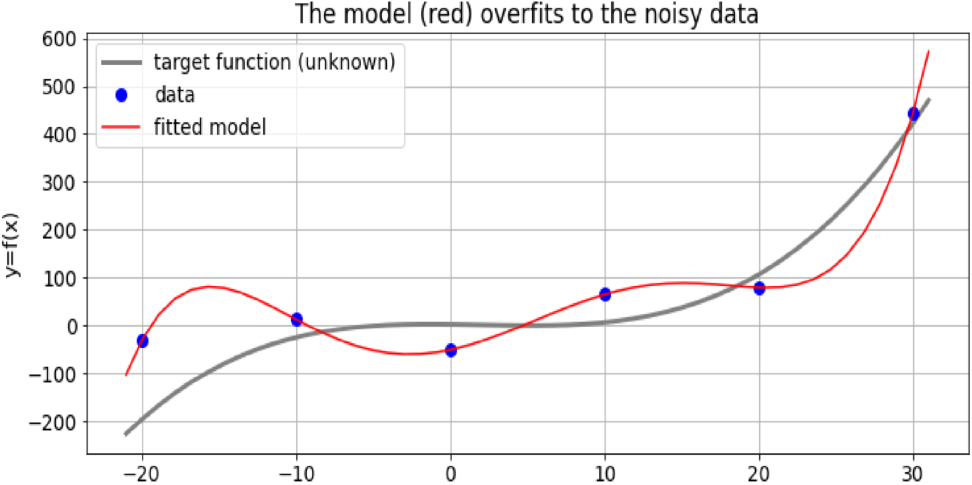
\includegraphics[width=0.9\linewidth]{./img/overfitting.png}

\subsection{Underfitting}
\begin{itemize}
    \item Using a too simple model
    \item In-Sample Error is large
    \item Generalization Error is large
    \item high bias and low variance
\end{itemize}

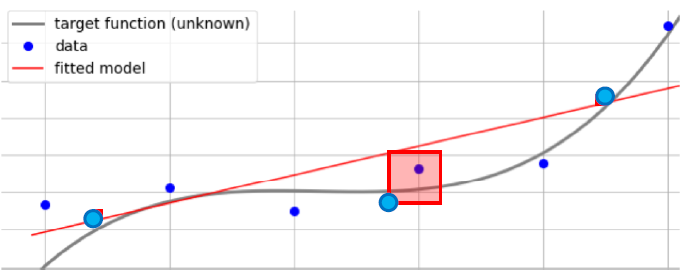
\includegraphics[width=0.9\linewidth]{./img/underfitting.png}

\subsection{Training-Set, Test-Set, Model Evaluation}
\CHECK{TE Titel besser 'Generalization Error'?}
\begin{itemize}
    \item Generalization Error: Der Fehler, den das Modell mit neuen (ungesehenen) Daten erziehlt.
    \item can't be calculated, but estimated (see Test-Error)
    \item Split the data into 2 sets: Training-Set (~80\% of data) \& Test-Set (~20\% of data)
\end{itemize}
\textbf{Training:} 
\begin{itemize}
    \item Fit the model to the training set. This minimizes the \textbf{in-sample error}
\end{itemize} 
\textbf{Evaluating:}
\begin{itemize}
    \item Using the Test-Set produces the \textbf{Test-Error (aka out-of-sample-error)}
    \item This is an estimate of the Generalization Error!
\end{itemize}

\subsection{Bias-Variance Trade-off}
\textbf{Variance (Streuung):} Difference of fits between data sets. Wie hoch ist die Streuung/Abweichung mit neuen Daten. Genauer: Wie gross ist der Unterschied bei verschiedenen Testsets (ungesehenen Daten)? Wenn die alle ''gleich gut/schlecht'' performen ist die Variance klein=besser. (Wie gut spielt also keine Rolle, nur wie gross die Unterschiede sind!). High Variance $\rightarrow$ Overfitting  

\textbf{Bias (Verzerrung):} Results that are systematically prejudiced due to faulty assumptions. Wie gut matcht mein Modell das ''echte Modell'' (Wirklichkeit)? High Bias $\rightarrow$ Modell zu einfach.

\textbf{High Bias}
\begin{itemize}
    \item A too simple model for the given data
\end{itemize}
\textbf{Low Variance}
\begin{itemize}
    \item The model is relatively stable
    \item Very simular model if trained with new data
\end{itemize}
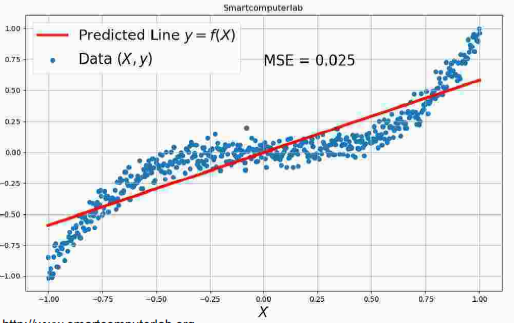
\includegraphics[width=0.6\linewidth]{./img/bias_variance.png}\\
\textbf{Low Bias}
\begin{itemize}
    \item A more complex model can better explain the data
\end{itemize}
\textbf{High Variance}
\begin{itemize}
    \item Given a new datapoint, the MSE can be very large
    \item For a different set with more datapoints, the model may be very different
\end{itemize}
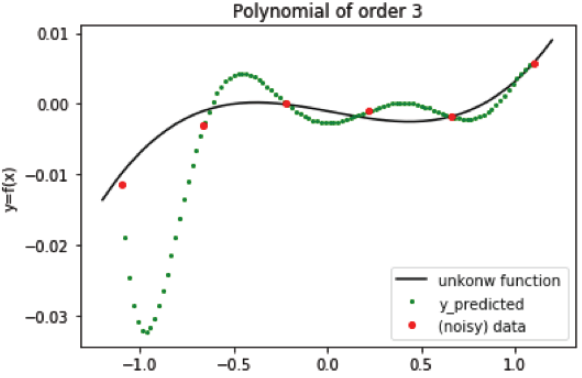
\includegraphics[width=0.6\linewidth]{./img/bias_variance2.png}

\subsubsection{Trade-off}
\begin{itemize}
    \item Higher bias implies lower variance
    \item Lower bias implies higher variance
    \item In practice, all we want is low variance
    \item The model can only be as complex as the data permits
    \item You have to find an optimal balance between bias and variance
\end{itemize}
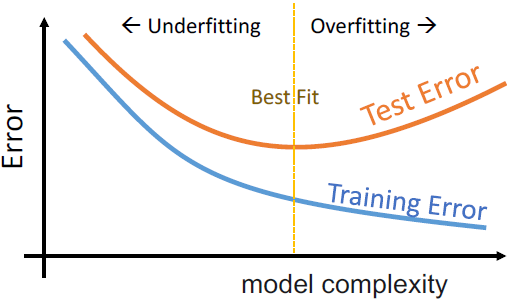
\includegraphics[width=0.6\linewidth]{./img/tradeoff.png}

\subsection{Regularization}
Geht immer um die freien Parameter des Modells. Man bestraft diese. 
\begin{itemize}
    \item Je einfacher das Modell, desto schlechter die Erklärung/ je komplexer das Modell, desto besser die Erklärung
    \item Technique to control the model complexity
    \begin{itemize}
        \item Add a penalty term to the Loss
        \item More complex models get a higher penalty
        \item when 2 models are equal $\rightarrow$ choose the simpler one (Occoams Razor)
        \item Add a constrain to the optimization process
        \item \textit{regularized loss} = \textit{MSE + $\lambda$ model-complexity}
    \end{itemize}
\end{itemize}
\begin{center}
    $\displaystyle\sum_{i = 1}^{n} (y_i - \displaystyle\sum_{j = 1}^{p} x_{ij}\beta_j)^2 + \lambda \displaystyle\sum_{j = 1}^{p}\beta_j^2$
\end{center}
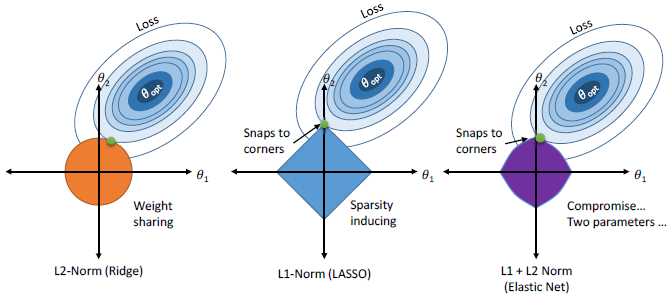
\includegraphics[width=1\linewidth]{./img/regularization.png}

\subsubsection{L1 Regularization}
\begin{itemize}
    \item Absolute Value
    \item Lasso Regression
    \item $mse = \frac{1}{n}\sum_{i=1}^{n} (y_i - h_{\theta}(x_i))^2+\textcolor{red}{\lambda \displaystyle\sum_{i=1}^n|\theta_i|}$
\end{itemize}

\subsubsection{L2 Regularization}
\begin{itemize}
    \item Quadriertes $\theta$
    \item Ridge Regression
    \item $mse = \frac{1}{n}\sum_{i=1}^{n} (y_i - h_{\theta}(x_i))^2+\textcolor{red}{\lambda \displaystyle\sum_{i=1}^n\theta_i^2}$
\end{itemize}

\subsubsection{L1 vs. L2 Regularization}
\begin{itemize}
    \item L1-Regularisierung versucht den Median der Daten zu schätzen
    \item L2-Regularisierung versucht den Mittelwert der Daten zu schätzen, um ein Overfitting zu vermeiden
    \item L1/L2-Norm bestrafen die Modellkomplexität
    \item $\lambda$ legt Verhältnis zwischen Bestrafung und Loss-Function fest
    \begin{itemize}
        \item $\lambda$ = 0 $\rightarrow$ nur Loss-Function relevant ("Bestrafung" = 0)
    \end{itemize}
    \item Entweder einfaches Modell oder komplexeres Modell nehmen und dieses via Generalisierung/ Optimization bestrafen
    \begin{itemize}
        \item zu Beginn gewähltes Modell ist fix/ starr
        \item Mit Generalisierung/ Regluarisierung kann dieses trotzdem nachträglich no "getuned" werden
    \end{itemize}

\end{itemize}


\subsection{Optimization with Keras / Tensorflow}
\begin{minted}{python}
    import tensorflow as tf
    from tensorflow import keras
    from tensorflow.keras import layers
    from tensorflow.keras import regularizers
    model = tf.keras.models.Sequential()
    # define the input. we provide the dimensionality of the input: poly_order
    inputs = keras.Input(shape=(poly_order_MODEL,))
    model.add(inputs)
    output_layer = layers.Dense(1, activation=None, use_bias=True, kernel_regularizer=regularizers.l2(0.005))
    model.add(output_layer)
    # Optimizer
    model.compile(optimizer=keras.optimizers.Adam(learning_rate=0.04),
    loss=keras.losses.MSE, # loss function to minimize
    metrics=[keras.metrics.MSE]) # list of metrics to monitor
\end{minted}

\TODO{Beispiel aus Übung week8\_regularization 'Define a neural network using Keras'}
        \section{Cross-Validation}
Alle Daten werden fürs Training sowie fürs Testing benutzt und daraus kann das optimale Modell/ Methode für das bestehende Problem ausgewählt werden.
Falls z.B. nur die ersten 75\% fürs Training und die letzten 25\% für Testing verwendet würden, kann nicht garantiert werden ob das Modell wirklich gut ist. In den letzten 25\% könnte es Ausreisser haben, welche das Ergebnis verfälschen würden.\\
\textbf{Problem with 80/20 Data Separation}
\begin{itemize}
    \item Test Error depends on random set
    \item For different Set, the test error would be different
\end{itemize}
With Cross-Validation we can obtain a \textbf{better estimate of the generalization error}

\subsection{k-fold Cross-Validation}
Bei der k-fold Cross-Validation werden die Daten in ''k'' Blöcke (aka Folds) aufgeteilt.\\

\subsubsection{Without k-Fold Cross-Validation}
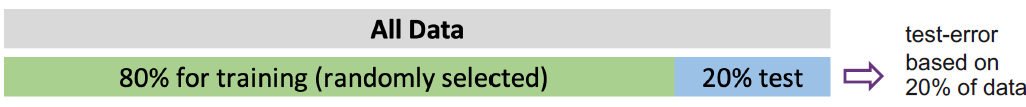
\includegraphics[width=\linewidth]{./img/k_fold.png}

\subsubsection{With k-Fold Cross-Validation}
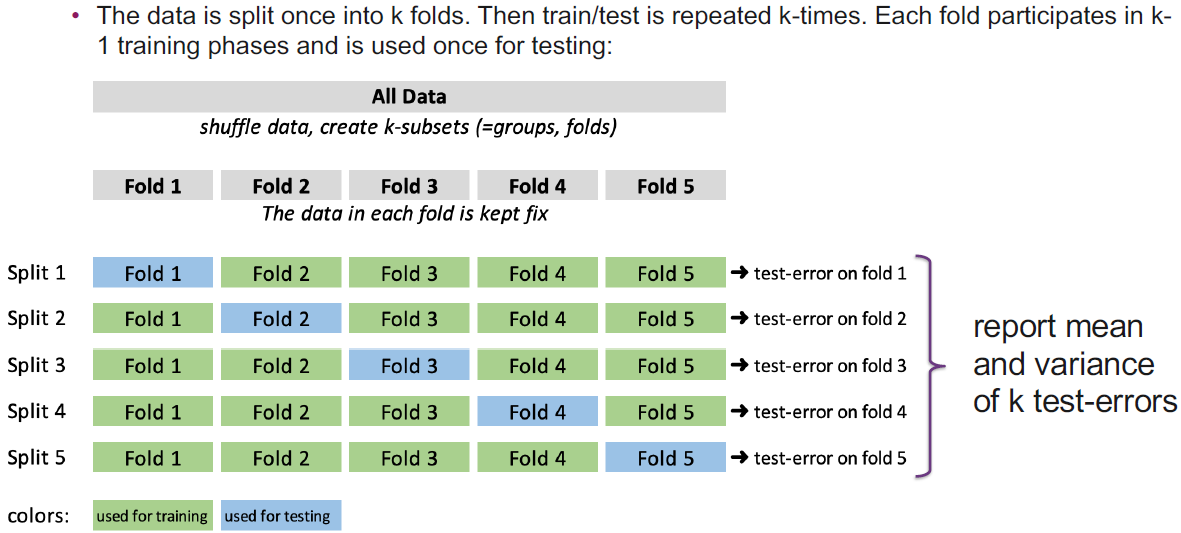
\includegraphics[width=\linewidth]{./img/k_fold2.png}

\subsubsection{Implementation}
\begin{minted}{python}
data = array([1, 2, 3, 4, 5,6]) # data sample
kfold = KFold(n_splits=3, shuffle=True, random_state=1) # prepare cross validation
for train, test in kfold.split(data): # enumerate splits
    print('train: %s, test: %s' % (data[train], data[test]))
# Output:
train: [1, 4, 5, 6], test: [2, 3]
train: [2, 3, 4, 6], test: [1, 5]
train: [1, 2, 3, 5], test: [4, 6]
\end{minted}

\subsubsection{Some Comments}
\begin{itemize}
    \item Typical Values for k are \textit{5,10} or \textit{N}
    \item The data of a fold does not change during procedure
    \item Do not preprocess the whole dataset
    \item Apply the preprocessing pipe-line to each split
\end{itemize}

\section{Artificial Neural Networks (ANN)}
\subsection{Artificial Neurons}
\begin{itemize}
    \item Receives an input vector $[x_1,x_2, ...]$
    \item Each neuron has its own input weights $[w_1, w_2, ...]$ and \textbf{bias} $b$
    \item Calculates the sum of the \textbf{weighted input} (\textit{}{dot product} $\vec{x} * \vec{w}$)
    \item and adds a \textbf{bias} $b$. Then passes the result through a nonlinear activiation function
    \item Be careful when adding more and more neurons to the network: each neuron adds free parameters to the model! We quickly have more parameters than data points, which yields overfitting. 
\end{itemize}
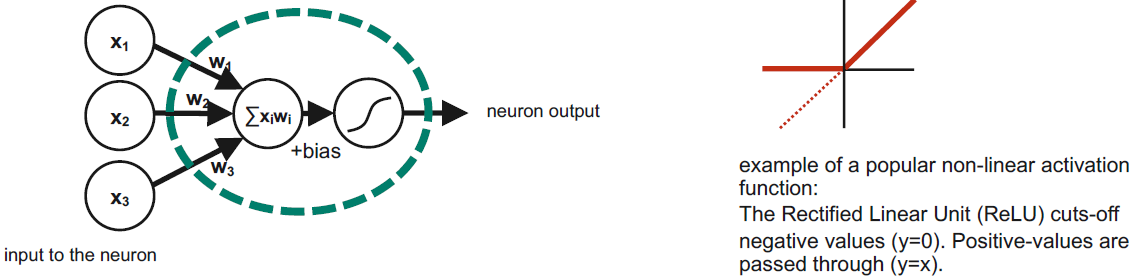
\includegraphics[width=\linewidth]{./img/artificial_neurons.png}

\subsection{Simple ANN}
Computer science definition von ANN:
\begin{itemize}
    \item  ANN ist eine Datenstruktur um eine beliebig komplexe mathematische Formel zu definieren
	\item  ANN ist eine Komposition von relativ simplen Expressions
    \item  ANN ist also wie ein Expression Tree (Root=Output / Leaves=Inputs)
\end{itemize}

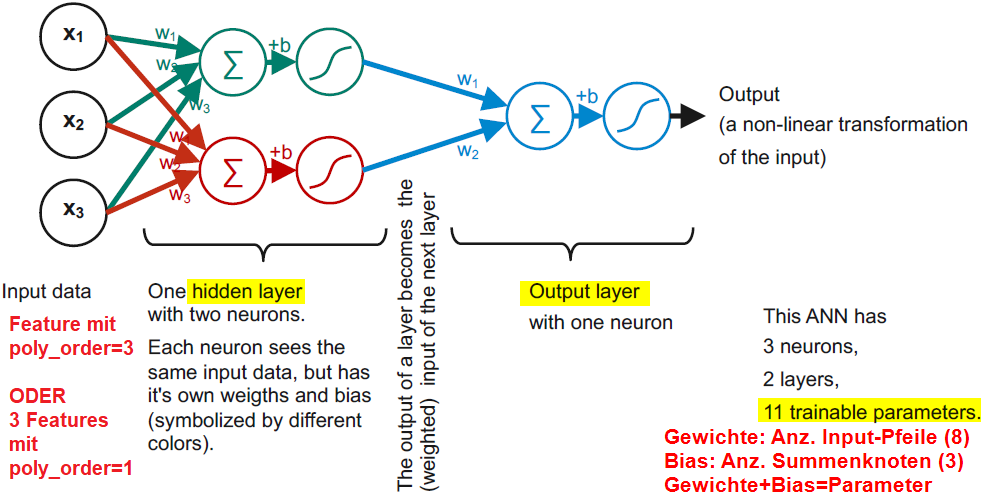
\includegraphics[width=\linewidth]{./img/ann_with_marks.png}
\begin{itemize}
    \item \textbf{Gewicht}: Anzahl Input-Pfeile (hier: 8)
    \item \textbf{Bias}: Anzahl Summenknoten (hier: 3)
    \item \textbf{Trainable Parameters}: Gewicht + Bias (hier: 11)
\end{itemize}

\begin{minted}{python}
poly_order_MODEL = 3 # => order_poly * features = nr of inputs
model = tf.keras.models.Sequential()

# define the input. we provide the dimensionality of the input: poly_order
inputs = keras.Input(shape=(poly_order_MODEL,))
model.add(inputs)

hidden_layer = layers.Dense(2, activation=activations.relu, use_bias=True, kernel_regularizer=regularizers.l2(0.0))
model.add(hidden_layer)

output_layer = layers.Dense(1, activation=activations.relu, use_bias=True, kernel_regularizer=regularizers.l2(0.0))
model.add(output_layer)
\end{minted}
\begin{minted}{text}
--> output
Model: "sequential"
 Layer (type)                Output Shape              Param #   
=================================================================
 dense (Dense)               (None, 2)                 8         
 dense_1 (Dense)             (None, 1)                 3         
=================================================================
Total params: 11
Trainable params: 11
Non-trainable params: 0
\end{minted}

\subsection{Traning an ANN}
\textbf{Supervised learning}
\begin{itemize}
    \item For each input $\vec{x}$ we are given the output $\vec{y}$
    \item ANN is initialized with random weights
    \item An optimizer reduces a cost-function (e.g. MSE)
    \item At every iteration, and for every single weight $w$ and bias $b$, the partial derivative needs to be calculated. (Backpropagation)
\end{itemize}
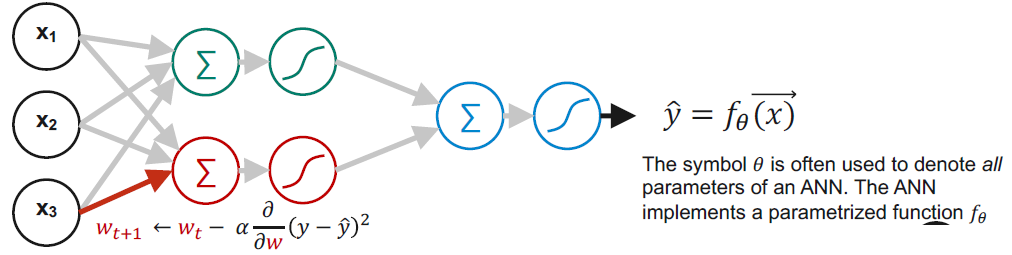
\includegraphics[width=\linewidth]{./img/train_ann.png}

\subsection{Backpropagation}
\begin{itemize}
    \item algorithm is used to effectively train a neural network through a method called chain rule
    \item after each forward pass through a network, backpropagation performs a backward pass while adjusting the model’s parameters (weights and biases)
\end{itemize}

\subsection{Activation Function: ReLu (Rectified Linear Unit)}

\begin{minipage}{0.5\linewidth}
\begin{itemize}
    \item linear function that will output the input directly if \txt{>0}, otherwise it will output 0
    \item default activation function formany types of neural networks, because a model that uses it is easier to train and often achieves better performance
    \item Possible Use Case: when we train the network to learn probabilities (values between 0 and 1)
\end{itemize}
\end{minipage}
\begin{minipage}{0.5\linewidth}
\begin{center}
    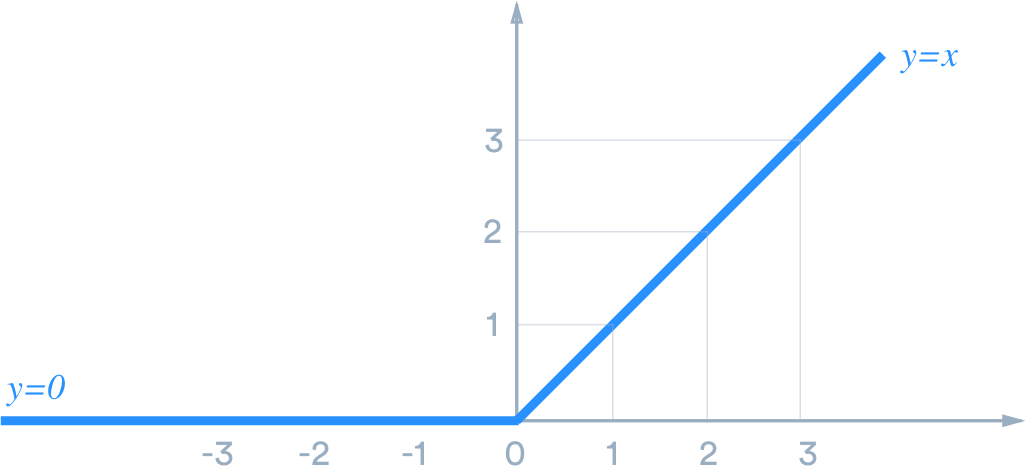
\includegraphics[width=\linewidth]{./img/relu.png}
\end{center}
\end{minipage}




\subsection{Single Input/ Output}
Wenn nur 1 Input vorhanden, dann ist der Input 1-Dimensional (alle Werte passen auf die X-Achse des Diagramms/ Graphen)
\begin{itemize}
    \item X-Achse: Input
    \item Y-Achse: Output
    \item Ergeben zusammen 2-Dimensionalen Graphen (X/Y-Achse)
\end{itemize}


        \section{Classification \& Logistic Regression}
\subsection{Binary Classification}
\begin{itemize}
    \item Decision with 2 possible outcomes
    \item Hail in Lausanne (yes/no)
    \item Master admission (admission / no admission)
    \item Based on different data / entity
\end{itemize}

\subsubsection{Decision using Linear Regression}
\begin{itemize}
    \item Train the model with gradient descent
    \item \textbf{Bad Idea!}
    \begin{itemize}
        \item The cost function minimizes the MSE difference in the values of $\hat{y}$ and $y$ and has nothing to do with the classification probabilities!
    \end{itemize}
    \item Models the response (y) and post process the response to compute the probability
\end{itemize}

\subsubsection{The sigmoid function}
\begin{center}
    $sigmoid(y) = \frac{1}{1 + e^{-y}}$
\end{center}
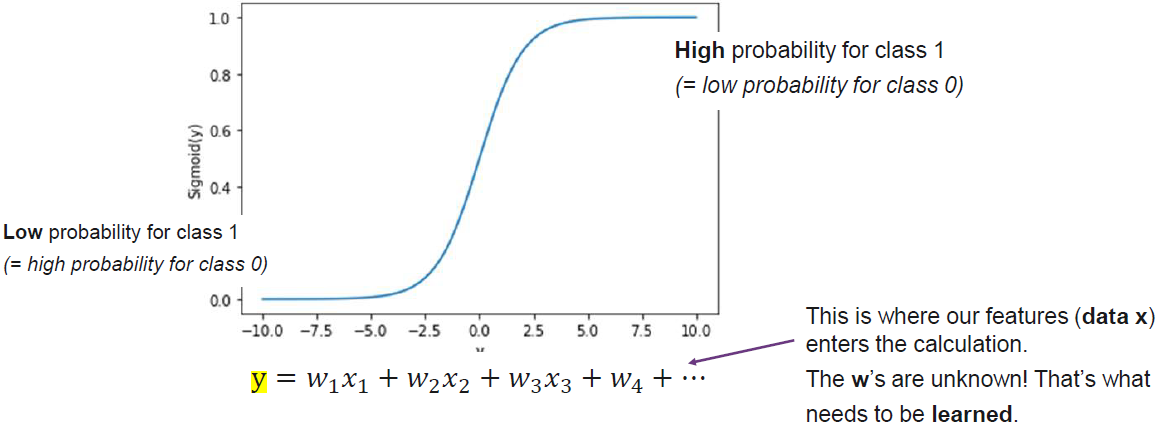
\includegraphics[width=\linewidth]{./img/sigmoid.png}

\textbf{Probabilities}\\
\begin{minipage}{0.59\linewidth}
\begin{itemize}
    \item We can write the estimated probability
    \item For a prediction we can write
\end{itemize}
\end{minipage}
\begin{minipage}{0.4\linewidth}
\begin{center}
    $P(x) = \frac{1}{1 + e^{-(W^{T}x)}}$
\end{center}
\end{minipage}

\textbf{Beispiel:}\\
How likely is it, that a student fit features $x_1=4.5$ and $x_2=5.5$ get accepted and get rejected?\\
\begin{center}
Parameters: $w_1=1, w_2=-0.7, w3=-0.7$\\
\end{center}
\begin{align*}
%$Features: x_1=4.5, x_2=5.5$\\
Pr(accept|x;w) &= \frac{1}{1 + e^{-(w_1*x_1+w_2*x_2+w_3)}} &= 0.49\\
Pr(reject|x;w) &= 1 - Pr(pass|x;w) &= 0.51
%($w_3$ ist wie ein 'Intercept')
\end{align*}

\subsubsection{Maximum Likelihood}
\begin{itemize}
    \item Given all the data points (X,Y) we want to maximize the probability that all the predictions are correct.
    \item For each of the training data, we want to maximize the likelihood of correct prediction
    \item We can use Gradient Descent to find W
\end{itemize}

\subsubsection{Maximum Likelihood Estimation (MLE)}
\textbf{Problem of Probability Density Estimation}
\begin{itemize}
    \item Density estimation is the problem of estimating the probability distribution for a sample of observations from a problem domain
    \item Common Solution $\rightarrow$ Maximum Likelihood Estimation (MLE)
\end{itemize}
\textbf{Maximum Likelihood Estimation (MLE)}
\begin{itemize}
    \item MLE involves defining a likelihood function for calculating the conditional probability of observing the data sample given a probability distribution and distribution parameters
    \item \textit{Goal}: find the optimal way to fit a distribution to the data
    \item MLE versucht den optimalen Wert für den Mittelwert oder die Standardabweichung einer Verteilung zu finden, wenn eine Reihe von Messwerten vorliegen
\end{itemize}
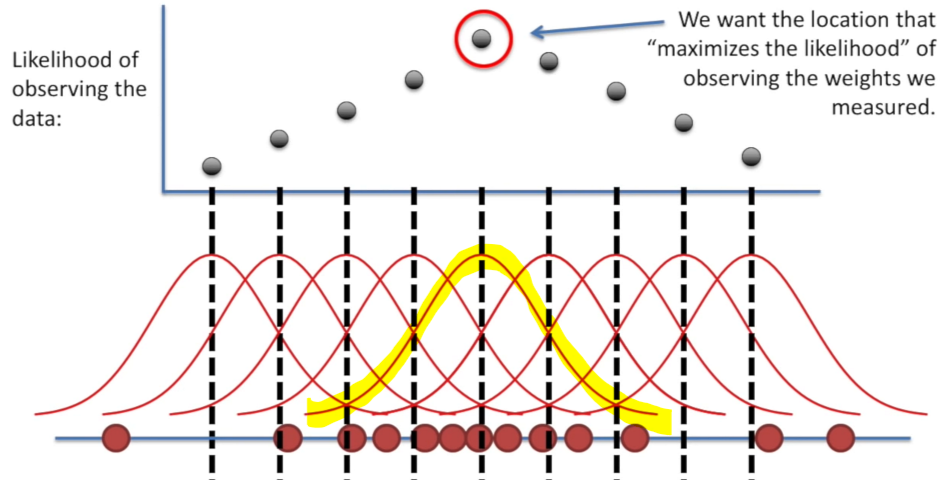
\includegraphics[width=\linewidth]{./img/mle.png}

\subsubsection{Loss Function used in logistic regression}
\begin{center}
    $\frac{-1}{N}\displaystyle\sum_{i = 1}^{N} y_i \ln(p_i) + (1 - y_i) \ln(1 - p_i)$
\end{center}

\subsection{Logistic Regression}
\begin{itemize}
    \item Die (binär) logistische Regressionsanalyse wird angewandt, wenn geprüft werden soll, ob ein Zusammenhang zwischen einer abhängigen binären Variablen und einer oder mehreren unabhängigen Variablen besteht.
    \item Mit binärerer logistic Regression können die Wahrscheinlichkeiten für das Eintreffen von Ereignissen vorausgesagt werden.
    \item Logistic Regression predicts whether something is \textbf{True} or \textbf{False}, instead of predicting something continuous like size (Linear Regression)
    \item Logistic Regression doesn't have the same concept of a "residual", so it can't use least squares and it can't calculate $R^2$
    \begin{itemize}
        \item Instead, it uses \textbf{mamimum likelihood}
    \end{itemize}
    \item \textit{Beispiel}:  Ausgang einer Aufnahmeprüfung $\rightarrow$ (Angenommen oder Abgelehnt = binäre logistic Regression (2 Möglichkeiten))
    \begin{itemize}
        \item Y-Achse: Wahrscheinlichkeit (1=sicher angenommen, 0=sicher abgelehnt)
        \item X-Achse: Intelligenz (je Intelligenter desto höher die Chance, angenommen zu werden)
        \item Je steiler die Kurve, desto besser die Vorhersage (des Prediktors)
    \end{itemize}
\end{itemize}

\begin{center}
    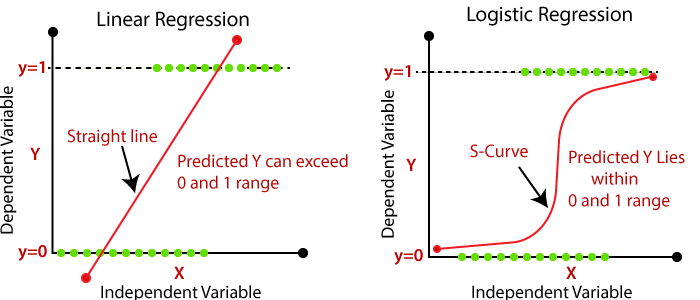
\includegraphics[width=0.8\linewidth]{./img/logistic_regression.png}
\end{center}

        \section{Classifier Evaluation}
\subsection{Confusion Matrix}
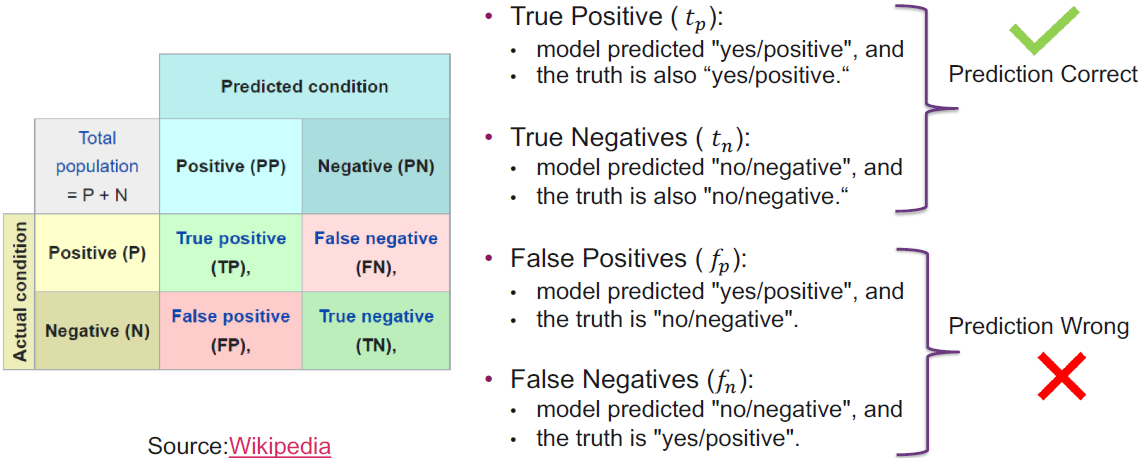
\includegraphics[width=\linewidth]{./img/confusion_matrix.png}
\textbf{Mean Accuracy:}
\begin{itemize}
    \item How often is the classifier correct?
    \item $A = (t_p + t_n) / n$
\end{itemize}
\textbf{Mean Error:}
\begin{itemize}
    \item How often is the classifier wrong?
    \item $E = (f_p + f_n) / n$
\end{itemize}
\textbf{Precision:}
\begin{itemize}
    \item When the prediction is 1, how often is it correct (True Positive)?
    \item $P = t_p / (t_p + f_p)$
\end{itemize}
\textbf{Sensitivity, Recall, True Positive Rate (TPR):}
\begin{itemize}
    \item How often the prediction is 1 when it's actually 1 (True Positive)
    \item $R = t_p / (t_p + f_n)$
\end{itemize}
\textbf{Miss Rate, False Negative Rate (FNR)}
\begin{itemize}
    \item $MR = 1 - TPR$
\end{itemize}
\textbf{Miss Rate, False Positive Rate (FPR)}
\begin{itemize}
    \item $R = f_p / (f_p + t_n)$
\end{itemize}

\subsection{Why Accuracy is not enough?}
\begin{itemize}
    \item If the prediction is constant the accuracy may still look decent
    \item E.g. always predict false
    \item 90\% of the data is false
    \item Accuracy = 90\% (decent)
    \item Precision = 0
    \item Recall = 0
\end{itemize}

\subsection{Precision vs. Recall}
\begin{itemize}
    \item Increasing precision reduces Recall and vice versa
    \item Threshold is a business decision (depending on goals)
\end{itemize}

\subsection{Receiver Operating Characteristics (ROC Curve)}
\begin{itemize}
    \item Defined by FPR and TPR as x and y axes
    \item Visualizes tradeoff between TPR (benefits) and FPR (cost)
\end{itemize}
\begin{center}
    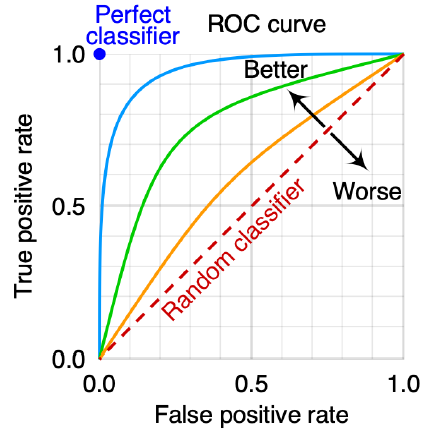
\includegraphics[width=0.4\linewidth]{./img/roc.png}
\end{center}
\textbf{Area under the curve}
\begin{itemize}
    \item Area under the ROC curve
    \item Shows how well the TPR and FPR is looking in the aggregate
    \item The greater the area under the curve, the higher the quality of the model
    \item The greater the area, the higher the ratio of TP to FP
\end{itemize}

\section{KNN}

\subsection{Linear Seperability (Decision Boundary)}
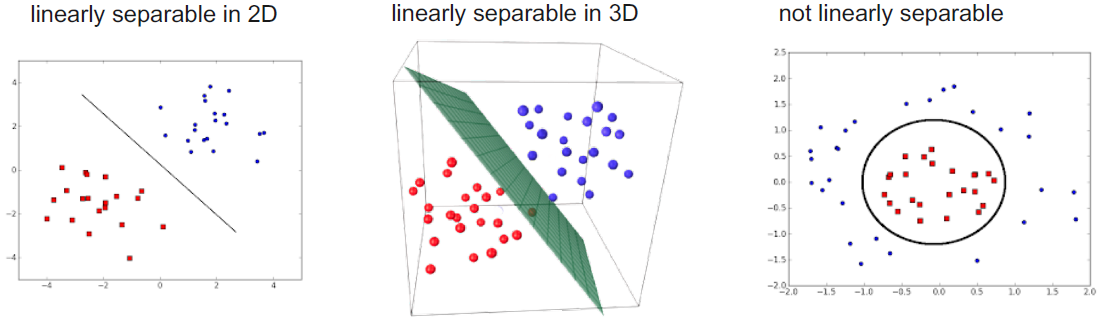
\includegraphics[width=1\linewidth]{./img/linear_sep.png}

\begin{itemize}
    \item Based on logistic regression model, you can draw a line
    \item This is the Linear decision boundary
    \item If a simple line perfectly seperates the classes, then the classes are said to be linearely seperable
\end{itemize}

\subsection{Non-Linear decision boundary}
\begin{itemize}
    \item When classes are not linearly seperable
    \item Resort to polynomial terms
\end{itemize}

\subsection{Multi-class classification}
\begin{itemize}
    \item e.g. COVID-Varianten, Weather-classes (sunny, cloudy, stormy..)
    \item Logistic Regresion can be extended One-vs-Rest (Cat/NoCat) / One-vs-One (Cat/Dog..)
    \item ...but slow training and can result in ambiguity. Therefore maybe KNN works better
\end{itemize}

\subsection{k-Neares Neighbors (KNN)}
\begin{itemize}
    \item super simple way to classify data (\textit{supervised learning})
    \item Works well for multi-class classification
    \item no complex training necessary, all data is used for each classification
    \item Basic Idea: A datapoint is know by the company it keeps
    \item Choose $k$ and compute distance to every neighbour for every datapoint
    \item Returns the most frequent class of the $k$ nearest neighbours\\
\end{itemize}
\textbf{Ablauf}
\begin{enumerate}
    \item Start with a dataset with known categories
    \item Add a new Datapoint or cell, with unknown category, to the cluster. We don't know this Datapoint's category because it was taken from another dataset where the Datapoints were not properly sorted
    \item We classify the new Datapoint by looking at the nearest annotated cells ("nearest neighbor)
    \begin{enumerate}
        \item If the \textit{k} in \textit{k-nearest neighbors} is equal to 1, then we only use the nearest neighbor to define the category
    \end{enumerate}
\end{enumerate}
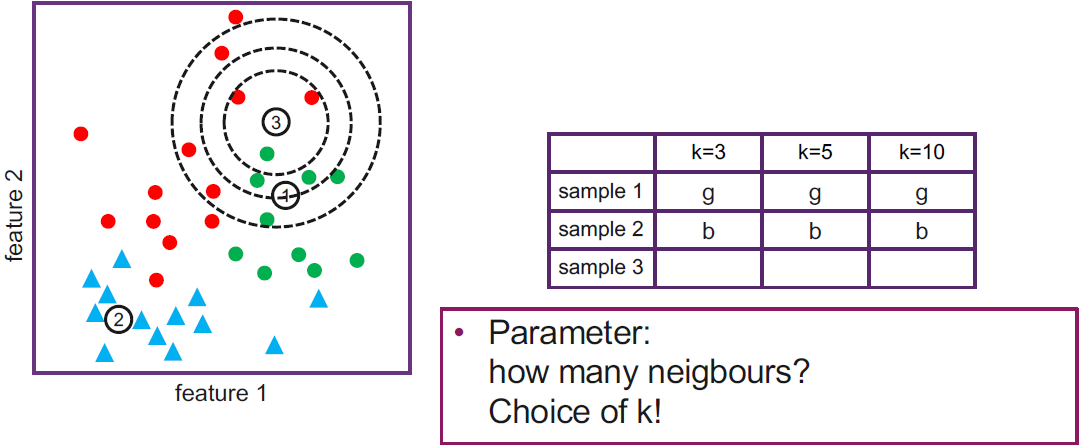
\includegraphics[width=0.8\linewidth]{./img/knn.png}
\subsubsection{Distance Metric}
\begin{itemize}
    \item Cosine Distance (Winkel)
    \begin{itemize}
        \item $\cos(\theta)=\frac{x_1 \cdot x_2}{|x_1| \cdot |x_2|}$
    \end{itemize}
    \item Manhattan Distance (Rhombus)
    \begin{itemize}
        \item $d_M=\displaystyle\sum_{i=1}^n | x_{1,n}-x_{2,n}|$
    \end{itemize}
    \item Euclidean Distance (most used, Kreis)
    \begin{itemize}
        \item $d_E=\sqrt{\displaystyle\sum_{i=1}^n(x_{1,n}-x_{2,n})^2}$
    \end{itemize}
    \item Minkowski Distance
\end{itemize}

\subsubsection{Choose of k}
\begin{itemize}
    \item if k is small, risk of overfitting (the decision boundary is dominated by only 1 datapoint)
    \item if k is big, risk of underfitting (decision boundaries are very smooth and cannot capture small differences that occur at the boundaries. Edge-cases are more likely to be misclassified)
    \item use confusion matrix the evaluate best k (e.g. precision and recall)
\end{itemize}

\subsubsection{Advantages}
\begin{itemize}
    \item Easy and simple ML model
    \begin{itemize}
        \item almost no training cost, but more calculating distance when used costs
    \end{itemize}
    \item Few hyperparameters to tune
\end{itemize}

\subsubsection{Disadvantages}
\begin{itemize}
    \item $k$ should be wisely selected (e.g. use cross-validation)
    \item Large computation cost during runtime if sample size is large
    \item Not efficient for high dimensional datasets
    \item Proper scaling should be provided for fair treatment among features
\end{itemize}

\subsubsection{Hyperparameters}
\begin{itemize}
    \item \textbf{K Value}: how many neighbours to participate in the KNN algo. If $k$ is to small = \textbf{overfitting} (fitting the noise) / if $k$ ist to large = \textbf{undefitting} (edge-casese more likely to be misclassified)
    \item \textbf{Distance Function}: Euclidean distance is most used
\end{itemize}

\subsection{Excercise}
\begin{minted}{python}
KNNclf = KNeighborsClassifier(n_neighbors=5, metric='euclidean')
KNNclf.fit(X_train, Y_train)
Y_hat = KNNclf.predict(X_test)
\end{minted}
\begin{itemize}
    \item For each different $k$, calculate accuracy, precision $tp/(tp+fp)$ and recall $tp/(tp+fn)$
    \item Which value of k would be your choose?
\end{itemize}
        \section{Clustering}
\subsection{Supervised Learning}
\begin{itemize}
    \item Supervised Learning ist ein Ansatz des maschinellen Lernens, der sich durch die Verwendung von markierten Datensätzen auszeichnet
    \item Diese Datensätze dienen dazu, Algorithmen zu trainieren oder zu "überwachen", damit sie Daten klassifizieren oder Ergebnisse genau vorhersagen können
    \item Anhand der beschrifteten Eingaben und Ausgaben kann das Modell seine Genauigkeit messen und mit der Zeit lernen
    \item kann beim Data Mining in zwei Arten von Problemen unterteilt werden: \textit{Classification} und \textit{Regression}\\
\end{itemize}

\textbf{Classification}:
\begin{itemize}
    \item Bei Klassifizierungsproblemen wird ein Algorithmus verwendet, um Testdaten genau in bestimmte Kategorien einzuordnen, z.B. um Äpfel von Orangen zu unterscheiden
    \item In der realen Welt können Algorithmen des überwachten Lernens verwendet werden, um Spam in einen separaten Ordner Ihres Posteingangs zu klassifizieren
    \item Lineare Klassifizierer, Support Vector Machines, Entscheidungsbäume und Random Forest sind allesamt gängige Arten von Klassifizierungsalgorithmen\\
\end{itemize}

\textbf{Regression}:
\begin{itemize}
    \item weitere Methode des supervised Learnings, die einen Algorithmus verwendet, um die Beziehung zwischen abhängigen und unabhängigen Variablen zu verstehen
    \item Regressionsmodelle sind hilfreich für die Vorhersage numerischer Werte auf der Grundlage verschiedener Datenpunkte, wie z. B. Umsatzprognosen für ein bestimmtes Unternehmen
    \item \textit{beliebte Algorithmen}: lineare Regression, die logistische Regression und die polynomiale Regression
\end{itemize}

\subsection{Unsupervised Learning}
\begin{itemize}
    \item We are given Data (features, x) without labels (y) \textbf{=unlabeled data}, an we still learn something from the data?
    \item Yes! Often the data has some structure. \textbf{The goal} of unsupervised learning is to self-discover patterns from the data (find hidden patterns in the data)
    \item Data without any structure is the exception. But the structure can be hidden by noise.
    \item Humans are extremely efficient at noting patterns. But algorithms are extremely efficient at dealing with large and high-dimensional datasets where humans fail
\end{itemize}

\subsection{What is clustering?}
\begin{itemize}
    \item Group $n$ data points into $k_c$ number of clusters
    \item the data points within a cluster should behave similar
    \item Underlying assumption: similar data points are ''close'' together
    \item Similar = Data points which have shared properties (similar features)
\end{itemize}

\subsubsection{Applications}
\begin{itemize}
    \item Social Network Analysis
    \item Astronomical Data
    \item Marked segmentation
    \item Recommendation systems
\end{itemize}

\subsection{Naive K-means}
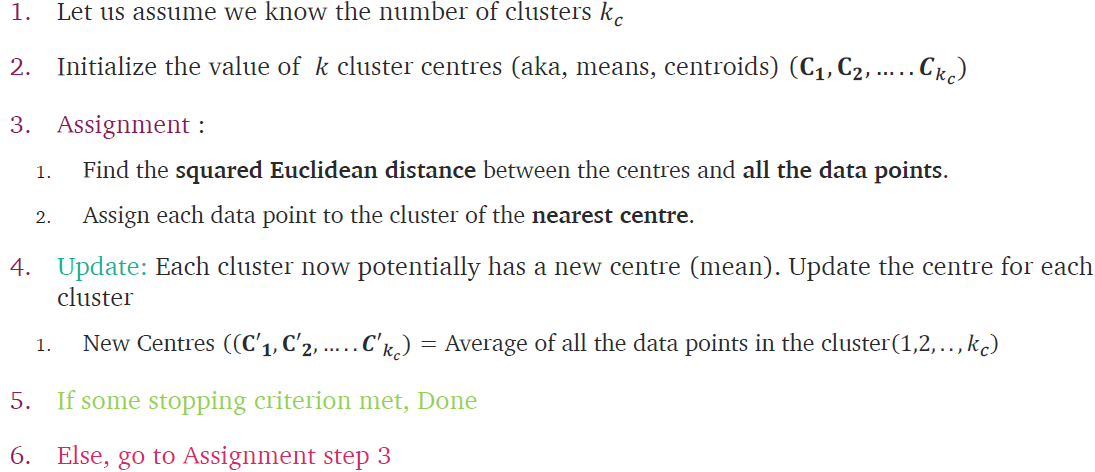
\includegraphics[width=\linewidth]{./img/k-means.png}
\subsection{K-Means Algorithm}
\begin{enumerate}
    \item Initially choose centers $C_1..C_{k_c}$ (can be random initialized)
    \item Assign step: Für alle Datenpunkte $j_1..N$ berechne die Distanz zu jeden Cluster-Center $C_1..C_{k_c}$. Dann jeder Datenpunkt dem Cluster zuordnen zu dem die Distance am geringsten ist
    \item Update step: Alle Center $C_1..C_{k_c}$ neu berechnen (mean of all data in cluster)
\end{enumerate}
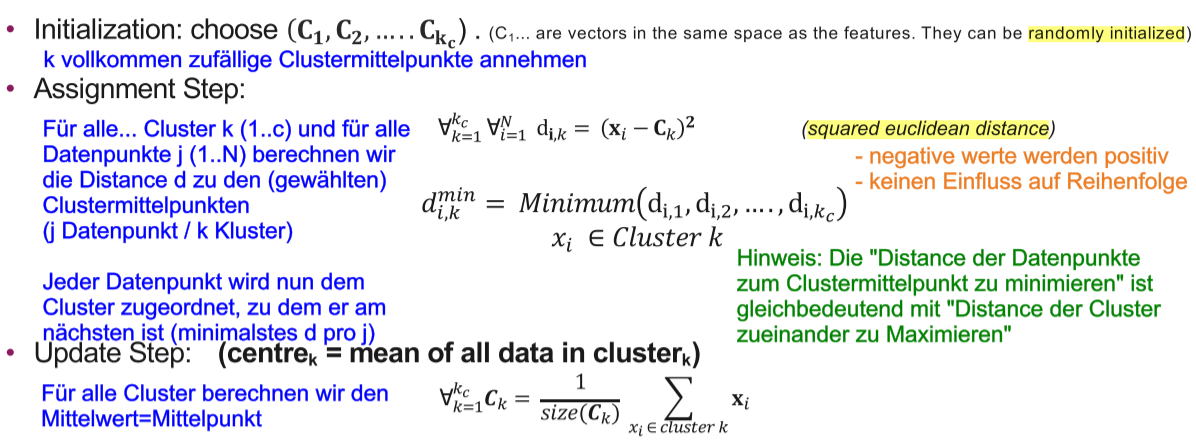
\includegraphics[width=\linewidth]{./img/w12_clustering_knn.png}

\subsubsection{Stopping Criterion}
\begin{itemize}
    \item When centres don't change (time consuming)
    \item The datapoints assigned to specific cluster remains the same (takes too much time)
    \item The distance of datapoints from their centres $>=$ treshold we have set
    \item Fixed number of iterations have reached (choose wisely)
\end{itemize}

\subsubsection{Initialization}
\begin{itemize}
    \item Performance depends on the random initialization
    \item Some seeds can result in a poor convergence rate
    \item Some seeds can converge to suboptimal clustering
    \item If centres are very close, it takes a lot of iterations to converge
    \item Initialize randomly, \textbf{run multiple times}
\end{itemize}

\subsubsection{Standardization of data (Scaling, Normalizing)}
\begin{itemize}
    \item Features with large values may dominate the distance value
    \item Features over small values will have no impact
    \item Normalize values! (Employ feature scaling with MinMaxScaler)
\end{itemize}
Verschiedene Skalierungen:
\begin{itemize}
    \item \textbf{Normalisierung} \python{MinMaxScaler}: Werte sind zwischen 0\dots1 (wichtig wenn Distanzen gerechnet werden)
    \item \textbf{Standardisieren} \python{StandardScaler}: Sodass Mittelwert=0 und Standardabweichung=1
    \item \textbf{Vector Normalisieren} \python{normalize}: Vector normalisieren auf Einheitsvektor (Länge $\sqrt{{x_1}^2 + {x_2}^2 + \dots}$ ergibt 1), macht das Rechnen einfacher resp. performanter
\end{itemize}

\subsection{Evaluation: Cluster Quality}
Choose the hyperparameter $k_c$ bigger than 1 and smaller than $N$. But what is a good values? Make clusters so that for each cluster the distance of each cluster member from its centre is minimized.

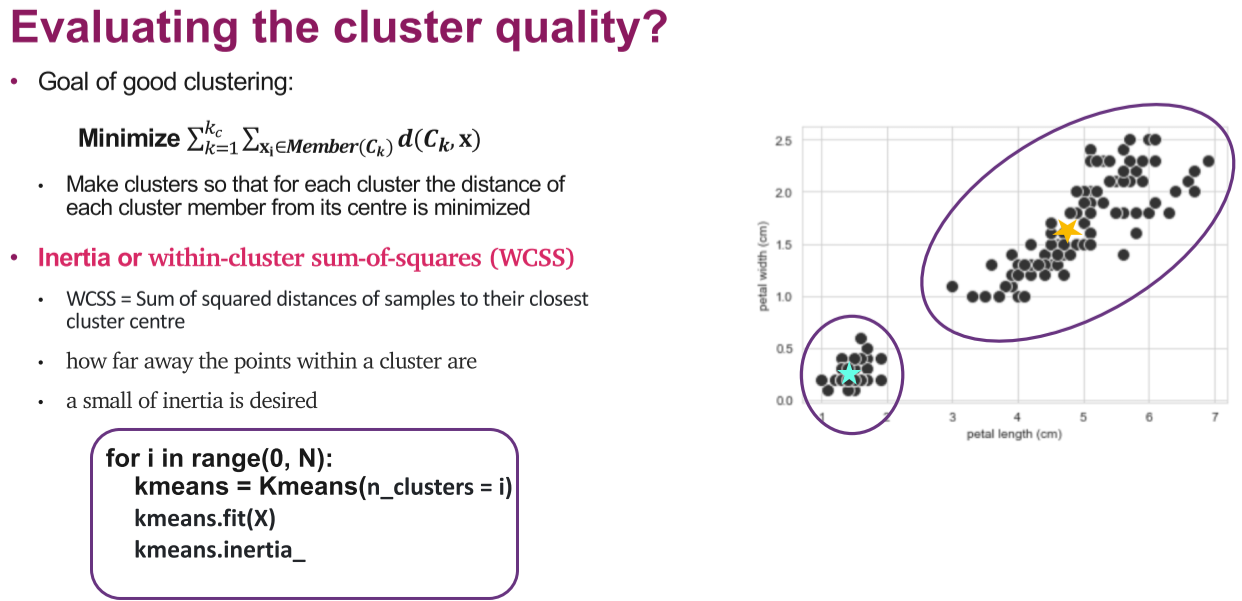
\includegraphics[width=\linewidth]{./img/w12_clusterquality.png}
\subsubsection{Inertia or within-cluster sum-of-squares (WCSS)}
\begin{itemize}
    \item Sum of squared distances to center
    \item ''Best'' cluster-size is where the ''elbow'' is (until sharp drop ends)
\end{itemize}
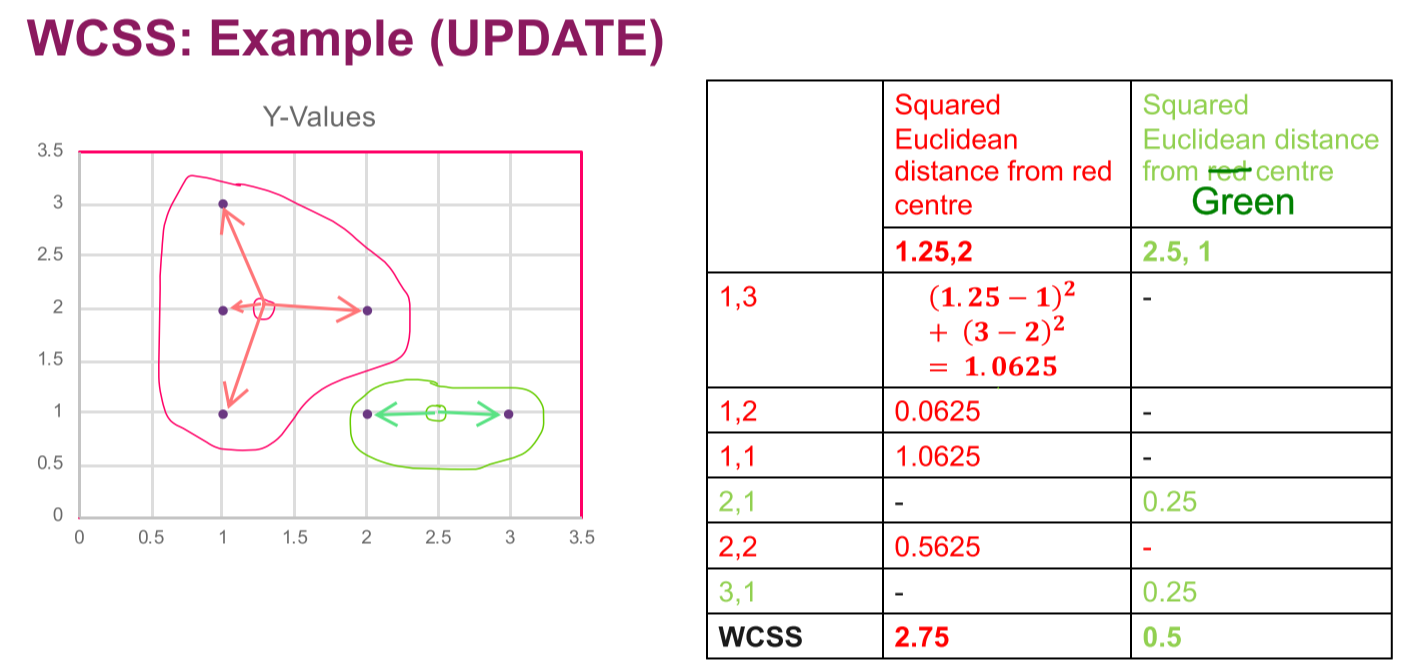
\includegraphics[width=\linewidth]{./img/w12_wcss.png}

\subsubsection{Silhouette Score}
\begin{itemize}
    \item \textbf{How far away the datapoints in one cluster are from the datapoints in another cluster}
    \item Silhouette Score of a point: $\frac{b-a}{max(a,b)}$
    \item $a$: average intra-cluster distance (distance between each point within)
    \item $b$: average inter-cluster distance (distance between a cluster and its nearest neighbour)
    \item Score should be close to 1 (good) and not close to -1 (bad)
    \item Silhouette Score of a cluster: mean of SS of each point in the cluster
\end{itemize}
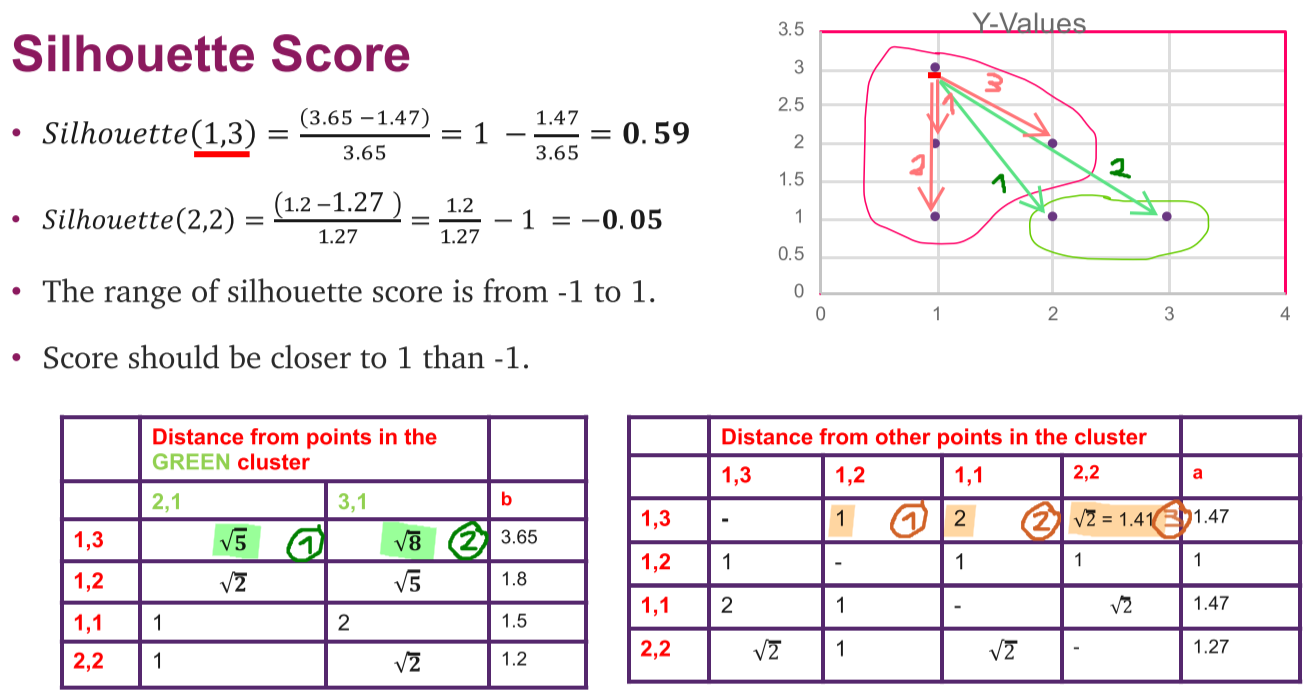
\includegraphics[width=\linewidth]{./img/w12_silhouette_score.png}

\subsubsection{How to choose number of clusters?}
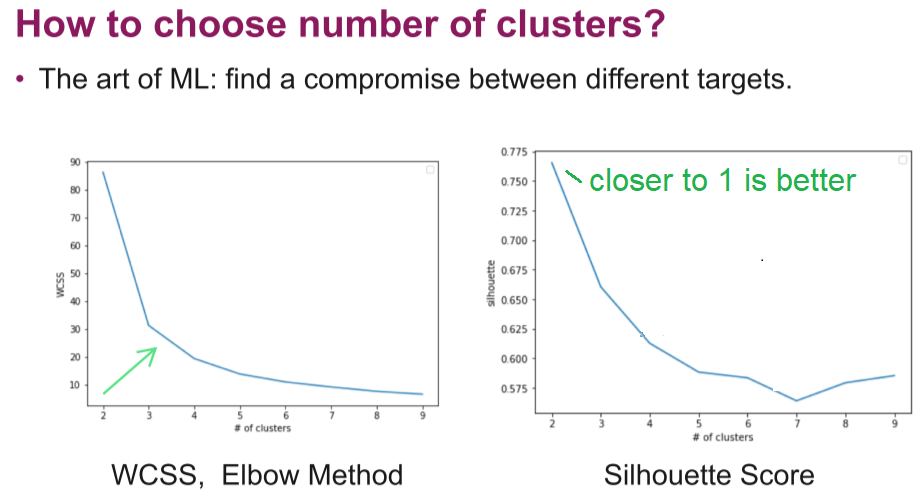
\includegraphics[width=\linewidth]{./img/w12_choose_nof_clusters.png}

\subsection{Implementation}
Aus sklearn-Folie: \python{from sklearn.preprocessing import MinMaxScaler} : data scaled wird aber in den Inclass-Notebooks niergends angewant (nur importiert)

\begin{minted}{python}
from sklearn.cluster import KMeans 
from sklearn.metrics import silhouette_score
from sklearn.preprocessing import normalize

#choose features
df = pd.DataFrame(iris.data, columns=iris.feature_names)
iris_3features = df.iloc[:, [0,1, 2]].values

kmeans = KMeans(n_clusters=2, init='k-means++', n_init=10, max_iter=300)
# - n_clusters = number of clusters (kc)
# - init = 'k-means++' selects initial cluster centers for k-mean clustering in a smart way to speed up convergence. 
# - max_iter = Number of iterations before stopping (stopping criterion)
# - n_init = Number of time the k-means algorithm will be run with different centroid seeds. 

# vector normalization
iris_3features= normalize(iris_3features)

# fitting the model to the data
kmeans.fit(iris_3features)

# output
print("cluster centres are", kmeans.cluster_centers_)
print("cluster labels of data points are", kmeans.labels_)
print ("Inertia is %f" %kmeans.inertia_)

# evaluate (different kc)
iterations = [], inertias = [], silhouettes = []
for k in range(kc_max):
  kmeans = KMeans(n_clusters=k)
  kmeans.fit(iris_3features)
  
  iterations.append(kmeans.n_iter_) #kmeans.n_iter_ is the number of iterations runs
  inertias.append(kmeans.inertia_)
  silhouettes.append(silhouette_score(iris_3features, preds))
\end{minted}
        \section{Ensemble Methods}
\subsection{Wisdom of Crowd}
\begin{itemize}
    \item Suppose you have a difficult question
    \item Ask many people and aggregate the answer
    \item This might work very well instead of finding the best suited person
\end{itemize}

\subsection{Ensemble}
\begin{itemize}
    \item Wisdom of Crowd can be applied to ML
    \item Instead of finding the best model, aggregate the results of weak models
    \item Aggregate predictions of regressors or classifiers
    \item Might get better accuracy than the best predictor
    \item Ensemble: group of predictors
\end{itemize}

\subsection{Ensemble Method}
\begin{itemize}
    \item Suppose we have many different weak models (better than random)
    \item Get prediction from all of them and take a vote
    \item Class with most votes is the predicted class
    \item Commonly used towards the end of a project
    \item \textbf{Requirement}: enough models / diverse models
\end{itemize}

\subsection{Different Dimensions}
Wo können überall Ensembles gemacht werden:
\begin{itemize}
    \item Different \textbf{algorithms} (e.g. KNN and Logistic Regression)
    \item Different \textbf{hyperparameters} (e.g. various k for KNN or regularization parameters for LR)
    \item Different training \textbf{data}: (e.g. cross validation, feature engineering, feature selection)
\end{itemize}

\subsection{Hard/Soft voting (final classification)}
\begin{itemize}
    \item \textbf{Hard voting:} Predict the class that gets the most votes
    \item \textbf{Hard voting:} Predict the class with the highest class probability, averaged over all classifiers (only possible if predictions are probabilities)
    \item Example using scikit-learn:
\end{itemize}
\begin{minted}{python}
log_clf = log_clf = LogisticRegression()
log_clf.fit(X_train, Y_train)
knn_clf = KNeighborsClassifier(n_neighbors= 3, metric=''Euclidean'')
knn_clf.fit(X_train, Y_train)
voting_clf = VotingClassifier(estimators=[ ('lr', log_clf), ('knn', knn_clf)], voting='hard') # estimators= two different models (k,v) | voting=hard
\end{minted}

\subsection{Bagging and Pasting}

\subsubsection{Bagging (Bootstrap Aggregating)}
\begin{itemize}
    \item Sampling \textbf{with replacement} (a data point can be selected more than once)
    \item durch das mehrfache verwenden einzelner Daten, kann das Modell stabilisiert werden
\end{itemize}

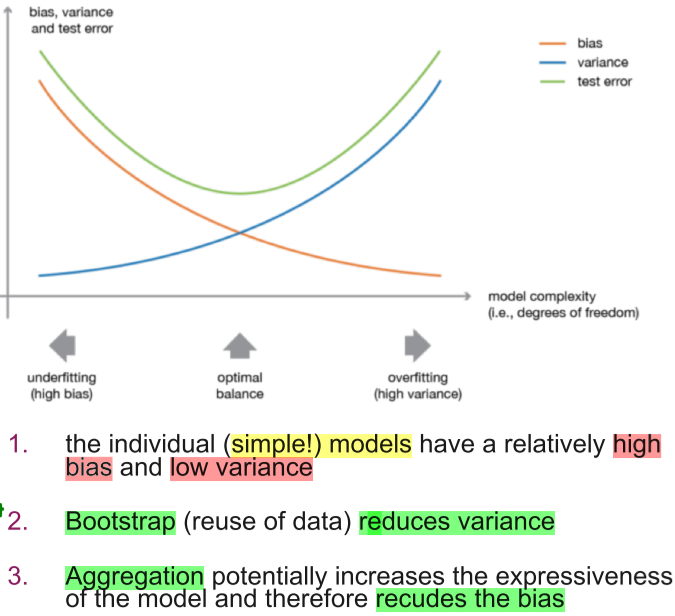
\includegraphics[width=0.75\linewidth]{./img/w13_bagging.png}

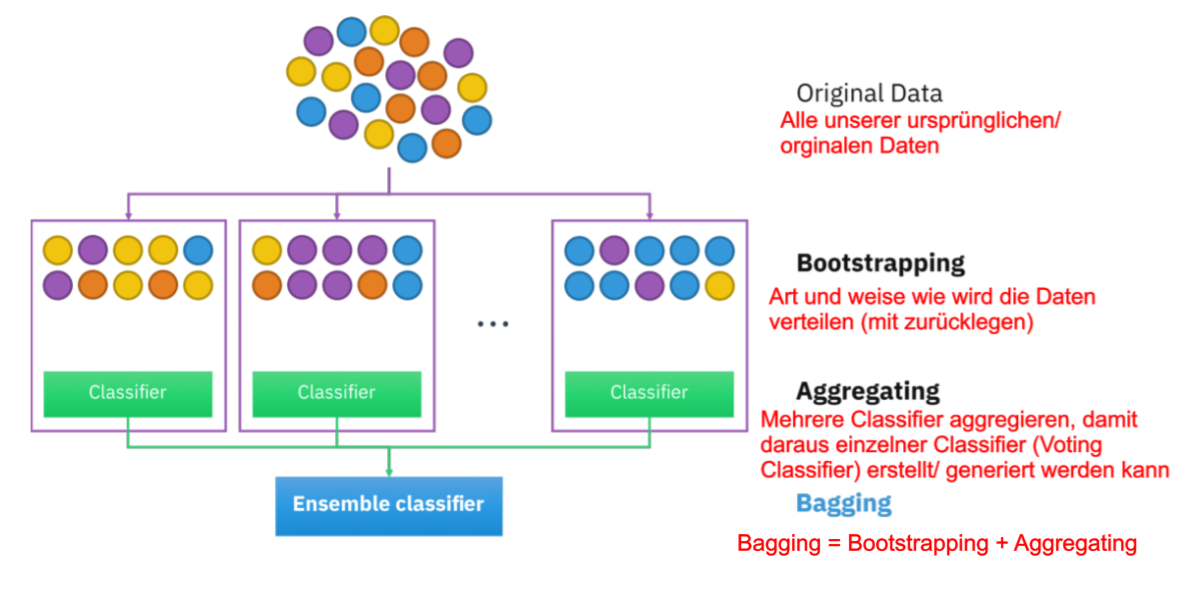
\includegraphics[width=\linewidth]{./img/bagging.png}

\subsubsection{Pasting}
In ML gibts nur Bagging, Pasting hat er nur als Gegenteil gebracht ist aber nicht relevant.
\begin{itemize}
    \item Wie Bagging nur: Sampling without replacement
\end{itemize}

\subsection{No free lunch theorem}
\textit{No single machine learning algorithm is universally the best-performing algorithm for all problems}
Some of the practical implications:
\begin{itemize}
    \item \textbf{No single algorithm} will solve all your machine learning problems better than every other algorithm
    \item Make sure you completely understand a machine learning problem and the data involved before selecting an algorithm to use
    \item All models are \textbf{only as good as the assumptions that they were created with} and the data that was used to train them
    \item \textbf{Simpler models like logistic regression have more bias and tend to \textit{underfit}, while more complex models like neural networks have more variance and tend to \textit{overfit}}
    \item The best models for a given problem are somewhere in the \textbf{middle of the two bias-variance extremes}
    \item To find a good model for a problem, you may have to \textbf{try different models and compare them using a robust cross-validation strategy}
\end{itemize}

\subsubsection{Training predictors (parallelization)}
\begin{itemize}
    \item If done sequentially can take too long. However, can be done in parallel!
    \item \python{ensemble_classifier = BaggingClassifier(..., n_jobs=-1) # -1=use all processors}
\end{itemize}

\subsubsection{Out of Bag (OOB) Evaluation}
Wenn Bagging verwendet wird, werden Werte eventuell mehrfach verwendet. Es kann aber auch Werte geben, welche gar nicht für das lernen verwendet wurden. Diese OOB-Daten sollen für die Überprüfung der Modelle angewendet werden.\\
\textbf{Vorteil:} Keine separate validation oder cross-validation nötig (aber es gibt am Schluss immer noch Test-Daten die gar nie verwendet wurden!)\\ 
\begin{minted}{python}
baggingRegressor = BaggingRegressor(base_estimator=LinearRegression(),
  n_estimators=50, 
  max_samples=0.05,  # each model is trained on 5% of the data (with replacement)
  max_features=6, # each model is sees only 6 (random) of 7 ftrs
  random_state=0, 
  oob_score = True # mit OOB
)
baggingRegressor = baggingRegressor.fit(X_train_scaled, y_train)

ensemble_classifier = BaggingClassifier(..., oob_score=True) # mit OOB
\end{minted}

\subsubsection{Different Features}
\begin{itemize}
    \item Different features can also be used for training predictors
    \item Bagging can be done on features as well
    \item Each predictor will be trained on  \textbf{random subesets} of the data features
    \item Sampling both features \& training data = \textbf{Random Patches}
    \item Sampling features only = \textbf{Random Subspaces}
\end{itemize}

\section{TI Befehle}
\begin{minipage}{0.5\linewidth}
\textbf{Skalarprodukt}
\begin{center}
    $Menu \rightarrow 7 \rightarrow C \rightarrow 3$\\
    $dotP\left(\begin{bmatrix}a \\ b\\ c\end{bmatrix}, \begin{bmatrix}d \\ e \\ f\end{bmatrix}\right)$
\end{center}
\end{minipage}
\begin{minipage}{0.49\linewidth}
\textbf{Normalisierungsvektor}
\begin{center}
    $Menu \rightarrow 7 \rightarrow 7 \rightarrow 1$\\
    $norm\left(\begin{bmatrix}a \\ b\\ c\end{bmatrix}\right)$
\end{center}
\end{minipage}

\begin{minipage}{0.5\linewidth}
\textbf{Ableiten/ Derivation}
\begin{center}
    $Menu \rightarrow 4 \rightarrow 1$\\
    $\frac{d}{dx}(5x)$
\end{center}
\end{minipage}
\begin{minipage}{0.49\linewidth}
\textbf{Integrieren}
\begin{center}
    $Menu \rightarrow 4 \rightarrow 3$\\
    $\int_{a}^{b} x^2,dx$
\end{center}
\end{minipage}

\textbf{Cosinus Distanz}
\begin{center}
    $cos(\theta) = \frac{dotP\left(\begin{bmatrix}a \\ b\\ c\end{bmatrix}, \begin{bmatrix}d \\ e \\ f\end{bmatrix}\right)}{norm\left(\begin{bmatrix}a \\ b\\ c\end{bmatrix}\right) * norm\left(\begin{bmatrix}d \\ e\\ f\end{bmatrix}\right)} \rightarrow Distanz (cos)$\\
    $\theta = cos^{-1}\left(\frac{dotP\left(\begin{bmatrix}a \\ b\\ c\end{bmatrix}, \begin{bmatrix}d \\ e \\ f\end{bmatrix}\right)}{norm\left(\begin{bmatrix}a \\ b\\ c\end{bmatrix}\right) * norm\left(\begin{bmatrix}d \\ e\\ f\end{bmatrix}\right)}\right) \rightarrow Distanz (Grad)$
\end{center}


    \end{multicols*}
\end{document}

























